\documentclass[11pt]{article}
\usepackage[T1]{fontenc}
\usepackage[utf8]{inputenc}
\usepackage[french]{babel}
\usepackage[margin=2.5cm]{geometry}
\usepackage{graphicx}
\usepackage{mathptmx}
\usepackage{setspace}
\usepackage{titlesec} 
\usepackage{imakeidx} 
\usepackage{tcolorbox}
\usepackage{caption}
\usepackage{verbatim}
\usepackage{pdfpages}
\usepackage[style=numeric]{biblatex}
\usepackage{enumitem}

\addbibresource{IR.bib}
\setlength{\parindent}{1cm}
\makeindex
\renewcommand{\rmdefault}{ptm}
\onehalfspacing % Interligne de 1.5
\setcounter{page}{1}
\titleformat{\section}
{\fontsize{16}{19}\selectfont\bfseries} 
{\thesection}
{20pt}
{}

\titleformat{\subsection}
{\fontsize{15}{19}\selectfont\bfseries} 
{\thesubsection}
{20pt}
{}

\renewcommand{\theparagraph}{\thesubsubsection.\arabic{paragraph}}
\titleformat{\paragraph}
{\normalfont\normalsize\bfseries}{\theparagraph}{1em}{}

% \makeatletter
% \renewcommand{\paragraph}{%
%   \@startsection{paragraph}{4}%
%   {\z@}{3.25ex \@plus1ex \@minus.2ex}{-1em}%
%   {\normalfont\normalsize\bfseries}%
% }
% \makeatother

\begin{document}
\pagenumbering{gobble} % Supprime la numérotation des pages
\begin{titlepage}
    \begin{center}

        \begin{minipage}[b]{0.3\textwidth}
            
\includegraphics[width=\textwidth]{images/Logo_Universite_de_Lorraine.png}
        \end{minipage}
        \begin{minipage}[b]{0.2\textwidth}
            \centering
            
\includegraphics[width=\textwidth]{images/logo-fst-format-jpg-couleur.jpg}
        \end{minipage}
        \smallbreak
        \vspace{0.5cm}
        \textbf{\large Master Informatique}

        %% Milieu de la page
        \vfill
        {\Large Reconnaissance des mouvements de la main} \smallbreak
        Rapport \smallbreak en vue de la validation de l'UE Initiation à la recherche \smallbreak
        \vfill
        \begin{tabular}{ccc|ccc}
            \'Etudiants : & Victor DALL\'E &  &  & Encadrante : & Madame BOLTCHEVA \\
                          & Claire KURTH   &  &  &              &
        \end{tabular}
    \end{center}

\end{titlepage}

\newpage \newpage
\section*{Décharge de responsabilité }\bigbreak
L'Université de Lorraine n'entend donner ni approbation  ni improbabtion aux opinions émises dans ce rapport,
ces opinions devant être considérées comme propres à leurs auteurs. \bigbreak

\newpage
\section*{Remerciements}
Nous souhaitons exprimer notre gratitude la plus sincère envers Madame Boltcheva pour son accompagnement, son soutien et son expertise tout au long de notre projet d'initiation à la recherche. Son engagement, sa patience et ses conseils précieux ont considérablement enrichi notre expérience et ont joué un rôle essentiel dans ce projet. Nous exprimons notre gratitude pour l'occasion qui nous a été offerte de collaborer avec elle, et nous exprimons notre profonde reconnaissance pour son engagement envers notre développement académique académique. Nous tenons aussi à exprimer notre reconnaissance envers nos familles, nos amis et tous ceux qui ont participé de près ou de loin à la concrétisation de ce projet. 

\newpage
\tableofcontents
\newpage

\pagenumbering{arabic}
\setcounter{page}{1}
\section*{Introduction}
\addcontentsline{toc}{section}{Introduction}
De nos jours, la vision par ordinateur est un domaine en plein essor. La reconnaissance de gestes fait partie intégrante de ce domaine et à ce titre, incarne une révolution dans la manière dont les utilisateurs interagissent avec les systèmes informatiques. Cette technologie est en effet en train de transformer la façon dont nous interagissont avec les machines. Cette avancée offre des opportunités novatrices dans des domaines tels que l'interaction entre l'homme et la machine,
la réalité augmentée ou encore l'accessibilité numérique.
De nombreuses techniques existent déjà pour permettre la détection des mains. MediaPipe de Google \cite{mediapipe} utilise le machine learning pour entrainer un modèle qui détecte les segments composant la main. D'autres travaux ont été réalisés comme ceux de l'équipe du professeur Kalpana Joshi \cite{joshi_static_2021} qui utilise les angles formés entre 2 doigts pour détecter la forme de la main (nombre de doigts, main ouverte ou fermée).\bigbreak

Contrairement aux interfaces traditionnelles basées sur le clavier et la souris, la reconnaissance des gestes permet aux utilisateurs de communiquer plus simplement avec les ordinateurs. Ils peuvent désormais avoir recours à leurs mains ou à leur corps pour contrôler les applications, ou encore naviguer dans des environnements virtuels. Cette approche favorise une expérience utilisateur plus immersive et ergonomique, ouvrant ainsi de nouvelles perspectives dans des domaines variés tels que le divertissement interactif, l'éducation, ou encore la médecine. Comme dit précédemment, la reconnaissance des mouvements joue un rôle crucial dans l’accessibilité numérique en permettant à des personnes porteuses d'un handicap physique  ou moteur de pouvoir communiquer et d'interagir avec des outils numériques plus facilement. En effet, celà permet de passer outre les obstacles liés à l’utilisation des outils traditionnels (tels que le clavier, la souris, la télécommande …) grâce à la simple utilisation de mouvements du corps. Cette nouvelle manière d'interagir avec un système numérique est déjà utilisée dans plusieurs domaines notamment le sport avec des applications de coaching personnel qui permettent de suivre les mouvements de l'utilisateur et ainsi lui donner des conseils pour améliorer sa technique, ou encore sa posture. Ce nouveau concept d'interraction permet également de pouvoir contrôler des appareils tels que des téléviseurs où par un simple geste, nous pouvons par exemple gérer le son ou changer de chaîne. \bigbreak

Dans ce contexte, ce projet vise à comprendre les mécanismes et problèmatiques liés à la reconnaissance des gestes de la main.
L'objectif principal est de concevoir un système capable de détecter et de classifier différents gestes de la main effectués par l'utilisateur,
tels que le poing fermé, ou alors la main ouverte avec un certains nombre de doigts levés. Ces gestes seront ensuite associés à différentes
actions telles que le lancement d'applications ou encore l'ouverture de sites web.
Pour réaliser ce projet nous utiliserons principalement la bibliothèque OpenCV. Nous parlerons dans un premier temps plus en détail des techniques de reconnaissance de gestes actuellement utilisées, puis nous verrons comment nous avons essayé de mettre en place notre système de reconnaissance de la main. Tout d'abord avec un classifieur Haar-cascade puis par traitement d'images. Nous verrons comment nous avons essayé de fusionner ces deux méthodes pour obtenir une meilleure détection de la main. Enfin, nous verrons comment nous avons essayé de détecter les mouvements de la main. 

\newpage

\section{Rappel du sujet et encadrement}
\subsection{Rappel du sujet}

Le but de ce projet est d’implémenter un système de reconnaissance des mouvements de la
main à l’aide d’un classifieur classique Haar-cascade. Le système doit reconnaître le geste de
la main de l’utilisateur (poing, un doigt, deux, trois, quatre,...) et le mapper à différentes tâches
telles que le lancement d’applications comme le bloc-notes, la peinture, et l’ouverture de sites web.
Le système doit être mis en œuvre avec l’aide de la librairie de "Computer Vision" - OpenCV,
comme dans l’article \cite{joshi_static_2021}. Une extension possible serait l’implémentation d’un système de détection
des mouvements de la tête ou du corps, tout entier.

\subsection{Encadrement}
Nous avons été encadré par Madame Boltcheva, enseignante-chercheuse à l'Université de Lorraine. Elle fait partie de l'équipe PIXEL du Laboratoire Lorrain de Recherche en Informatique et ses Applications (LORIA). Cette équipe fait de la recherche en traitement numérique de la géométrie et s'intéresse particulièrement aux techniques de paramétrisation, de maillage et de reconstruction d'objets à partir de nuages de points 3D.


\newpage

\section{\'Etat de l'art}
\subsection{Article de départ}
L'article sur lequel nous nous basons, \textit{Static Hand Gesture and Face Recognition System} \cite{joshi_static_2021} propose un système de reconnaissance de gestes de la main. Ce système est créé à partir d'une image, passée en HSV à laquelle ils ont ajouté un Flou et un Thresholding. Le Thresholding permet de généré une image binaire :  chaque pixel est comparé à un seuil, si la valeur du pixel est supérieur à ce seuil le pixel est blanc, sinon il est noir. Ils extraient ensuite les contours avant de tracer le Convex Hull, le polygone de la main. Enfin, ils calculent des "Convexity Defect" c'est-à-dire des points éloignés de points convexe. Dans ce cas ci, les points convexes sont le bout des doigts et donc les defects sont le trou entre 2 doigts. Un defect est donc compté si l'angle entre 2 doigts est supérieur à 90°. 

\subsection{Médiapipe}
Médiapipe est un framework open-source développé par Google permettant de construire des pipelines de traitement de données multimédia. Il propose des solutions pour la détection de la main, du visage ou encore de la pose. Il est basé sur des modèles de machine learning notamment grâce à de l'apprentissage via des réseaux de neurones. \bigbreak

\begin{center}
    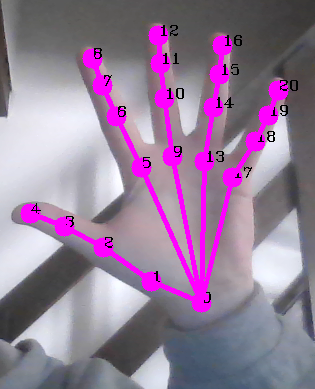
\includegraphics[width=0.5\textwidth]{images/mediapipe_ex.png}
    \captionof{figure}{Exemple de détection de la main avec Médiapipe}
\end{center}


\subsection{Classifieur Haar-cascade}
Le classifieur Haar-cascade est une méthode de détection d'objets dans une image introduit par Paul Viola et Michael Jones en 2001 \cite{viola_rapid_2001}. Il est basé sur l'utilisation de caractéristiques (ou features) de type Haar. Ces caractéristiques sont des fenêtres de taille fixe qui sont déplacées sur l'image et qui permettent de calculer la différence de luminosité entre les pixels de la fenêtre. Ces caractéristiques sont ensuite utilisées pour entraîner un classifieur qui permet de détecter des objets dans une image. \bigbreak

\begin{center}
    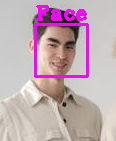
\includegraphics[width=0.2\textwidth]{images/visage.png}
    \captionof{figure}{Exemple de détection de visage avec un classifieur Haar-cascade}
    \label{fig:visage}
\end{center}

Les classifieurs Haar-cascade sont utilisés pour la détection de visages (Fig. \ref{fig:visage}), de voitures, de plaques d'immatriculation, de piétons, de mains ou de tout autres objets. Ils sont très utilisés dans le domaine de la vision par ordinateur et sont très efficaces pour la détection d'objets dans une image. 



\newpage

\section{Reconnaissance de la main avec un classifieur Haar-cascade}
\subsection{Entrainer un classifieur Haar-cascade}
Pour entrainer un classifieur Haar-cascade \cite{mittal_haar_2024}, il faut tout d'abord collecter des images positives et négatives. Les images positives sont des images contenant l'objet que l'on souhaite détecter, tandis que les images négatives sont des images ne contenant pas l'objet. Il faut ensuite générer des fichiers de descriptions des images positives et négatives. Ces fichiers contiennent les coordonnées des objets à détecter dans les images positives. Enfin, il faut entrainer le classifieur à l'aide de ces fichiers de descriptions. \bigbreak

L'entrainement du classifieurs en lui-même se fait grâce à ce que l'on appelle des "features". Ces dernières ont été introduites par Viola et Jones en 2001 (Fig. \ref{fig:haar_features_1}). Par la suite, d'autres features ont été ajoutées (Fig. \ref{fig:haar_features_2}) afin d'améliorer la détection d'objets dans une image.
\bigbreak \bigbreak

\begin{minipage}[t]{0.35\textwidth}
    \begin{center}
        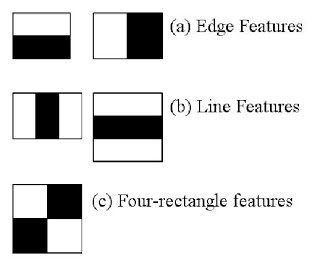
\includegraphics[width=\textwidth]{images/haar_features.jpg}
        \captionof{figure}{Features de Haar comme utilisées par Viola et Jones \cite{opencv}.}
        \label{fig:haar_features_1}
    \end{center}
\end{minipage}\hspace{1.5cm}
\begin{minipage}[t]{0.45\textwidth}
    \begin{center}
        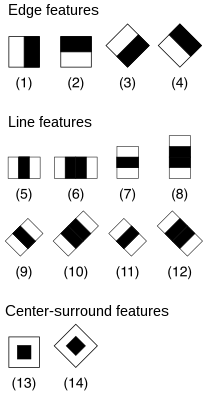
\includegraphics[width=0.8\textwidth]{images/haar_feature_2.jpg}
        \captionof{figure}{Features de Haar supplémentaires \cite{features_2}.}
        \label{fig:haar_features_2}
    \end{center}
\end{minipage}

\bigbreak \bigbreak


Ces features sont des caractéristiques de l'objet que l'on souhaite détecter, ce sont des patterns de pixels qui permettent de distinguer l'objet des autres éléments de l'image.

\noindent Il existe différents types de patterns :
\begin{itemize}[label=-]
    \item Les "edges" : ce sont des patterns qui permettent de détecter les contours de l'objet.
    \item Les "lines" : ce sont des patterns qui permettent de détecter les lignes de l'objet.
    \item Les "center-surrounder" : ce sont des patterns qui permettent de détecter les changements d'intensité entre le centre d'une région rectangulaire et le reste de la région. Cela permet de détecter des objets de forme particulière.
\end{itemize}

\bigbreak

Pour détecter ces patterns, l'algorithme utilise des fenêtres de taille fixe qui sont déplacées sur l'image. Ces fenêtres permettent de calculer la différence de luminosité entre les pixels de la fenêtre. Ces différences de luminosité sont ensuite utilisées pour déterminer si le pattern est présent dans l'image. 

\bigbreak

Ces features sont ensuite utilisées pour entrainer un classifieur qui permet de détecter l'objet dans une image. Le classifieur est entrainé à l'aide d'un algorithme de machine learning tel que AdaBoost \cite{adaboost} qui permet de déterminer les features les plus pertinentes pour la détection de l'objet. \bigbreak

AdaBoost est un algorithme d'apprentissage supervisé qui permet de construire un classifieur fort à partir de plusieurs classifieurs faibles.
Au début, chaque élément de la base de données à le même poids. L'algorithme va ensuite sélectionner un classifieur faible (par exemple, un arbre de décision simple) qui performe légèrement mieux que l'aléatoire. Ce classifieur va être utilisé pour prédire les éléments de la base de données. Les exemples mal classés reçoivent un poids plus élevé, tandis que les exemples correctement classés reçoivent un poids plus faible. Ainsi, les exemples difficiles à classer ont plus d'influence sur la formation du classifieur final. Les poids des classifieurs faibles sont déterminés en fonction de leur précision relative. Les classifieurs les plus précis ont un poids plus élevé. Enfin, le classifieur final est une combinaison linéaire des classifieurs faibles pondérés par leur précision relative.

\subsection{Nos entrainements}
\subsubsection{Avec une base de données d'images de mains}
\paragraph{Méthodologie}
Pour notre entrainement, nous avons collecté 10 000 images négatives (Fig. \ref{fig:ex_neg}) \cite{negatives, bdd_animal} et 5 000 images positives de mains (Fig. \ref{fig:ex_pos}) \cite{afifi201911kHands}. Nous avons dû pour les images positives, annoter les images (dans un fichier texte) afin de donner le nombre de mains présentes et les coordonnées de la main dans l'image (Fig. \ref{fig:ex_desc}). \'Etant donné que seule une main était présente et que le fond est blanc, la zone où est située la main est donc l'image entière. Ensuite, grâce à ce fichier et à OpenCV, nous avons généré un fichier vec qui contient les informations des images positives. Nous avons ensuite entrainé le classifieur à l'aide de ce fichiers.
\bigbreak


\begin{minipage}[t]{0.5\textwidth}
    \begin{center}
        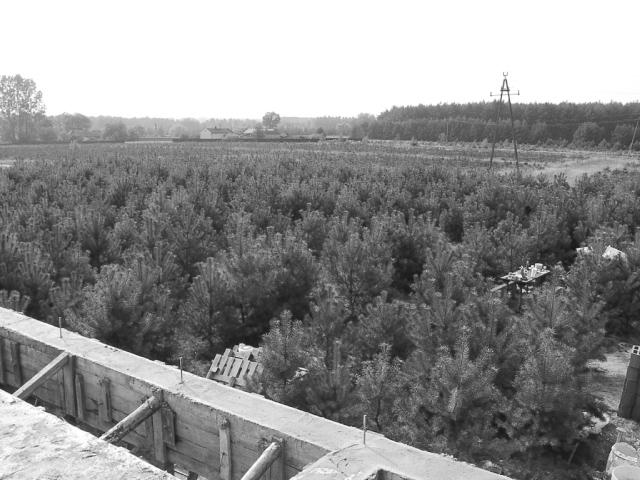
\includegraphics[width=0.5\textwidth]{images/ex_neg.jpg}
        \captionof{figure}{Exemple d'image négative}
        \label{fig:ex_neg}
    \end{center}
\end{minipage}
\begin{minipage}[t]{0.45\textwidth}
    \begin{center}
        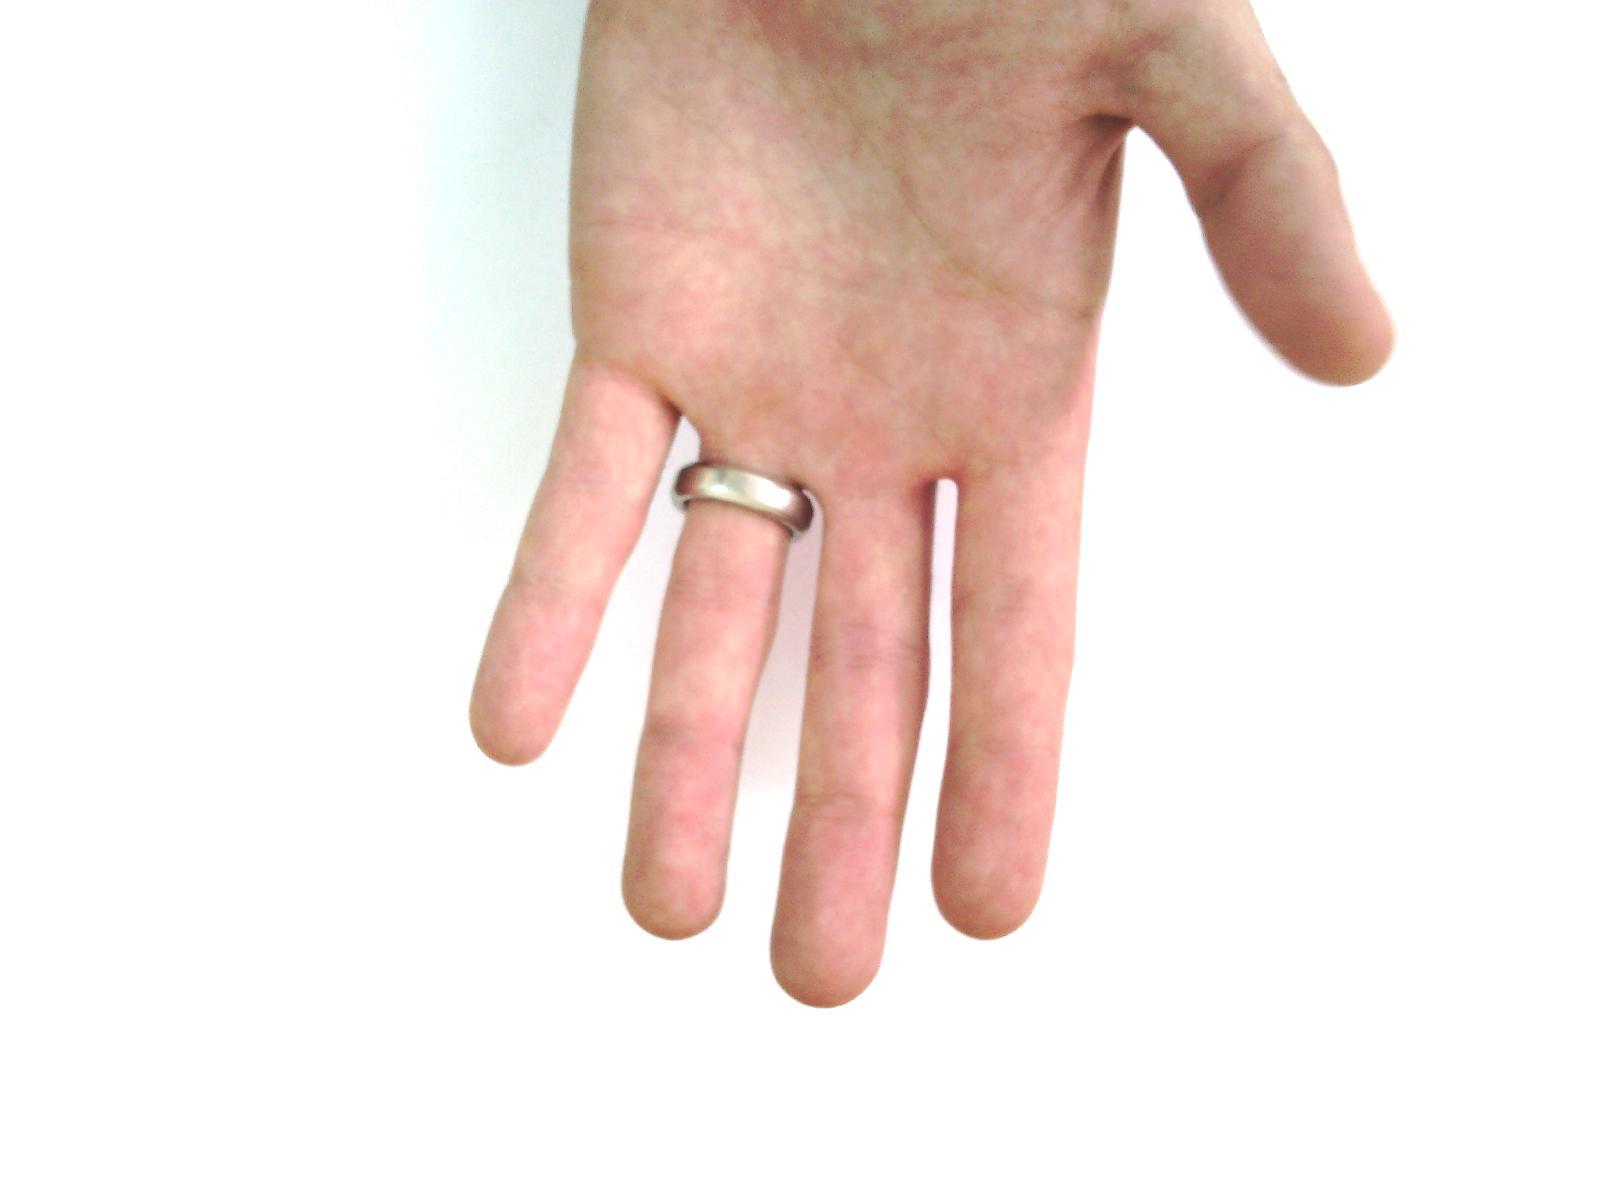
\includegraphics[width=0.5\textwidth]{images/ex_pos.jpg}
        \captionof{figure}{Exemeple d'image positive}
        \label{fig:ex_pos}
    \end{center}
\end{minipage}

\bigbreak \bigbreak \bigbreak

\begin{center}
    \begin{verbatim}
        positives\Hand_0000002.jpg 1 0 0 50 38
        positives\Hand_0000003.jpg 1 0 0 50 38
        positives\Hand_0000004.jpg 1 0 0 50 38
    \end{verbatim}
    \captionof{figure}{Exemple de fichier de description}
    \label{fig:ex_desc}
\end{center}


\bigbreak \bigbreak

Nous sommes ensuite passés à l'entrainement. Nous avons utilisé pour celà OpenCV \cite{opencv} qui propose un programme pour entrainer un classifieur Haar-cascade. Nous avons testé plusieurs cas : avec 5, 10, 15 et 20 étapes, avec des profondeurs d'arbres maximum différentes, avec plus d'images positives que négatives et inversement. Nous avons également testé différentes valeurs pour le seuil d'acceptation du ratio break. Ce seuil détermine à quel point le modèle continue à apprendre avec précision et quand il doit s'arrêter. Enfin, nous avons testés avec deux modes différents : par défaut et 'ALL'. Le mode par défaut utilisent les features de bases (Fig. \ref{fig:haar_features_1}) tandis que le mode 'ALL' utilisent les features un peu plus complexes (Fig. \ref{fig:haar_features_2}). \'A la fin de l'entrainement, nous récupérons un fichier xml qui sera ensuite utilisé pour la détection.\bigbreak

\bigbreak

\noindent Voici un tableau récapitulatif des différents tests que nous avons effectués : \bigbreak

\begin{center} 
    \begin{tabular}{|c|c|c|c|c|c|c|c|}
        \hline
        Test & Nombre de & Nombre de & Nombre & Profondeur & Acceptance  & Mode & Temps \\
        & positifs & négatifs & d'étapes & d'arbre & Ratio Break &  &  \\ 
        \hline 
        1 & 4 000 & 10 000 & 7 & 1 & désactivé & Défaut & 1h10 \\ 
        \hline
        2 & 4 000 & 10 000 & 8 & 1 & 1.0e-5 & Défaut & 40min \\
        \hline
        3 & 4 000 & 2 000 & 10 & 3 & 1.0e-5 & All & 5h \\
        \hline
        4 & 4 000 & 2 000 & 6 & 1 & 1.0e-5 & Défaut & 4mn \\
        \hline
    \end{tabular}
\end{center}

\bigbreak

\paragraph{Résultats}
Nous voulions obtenir un classifieur qui détecte la main dans une image comme suivant : 
\begin{center}
    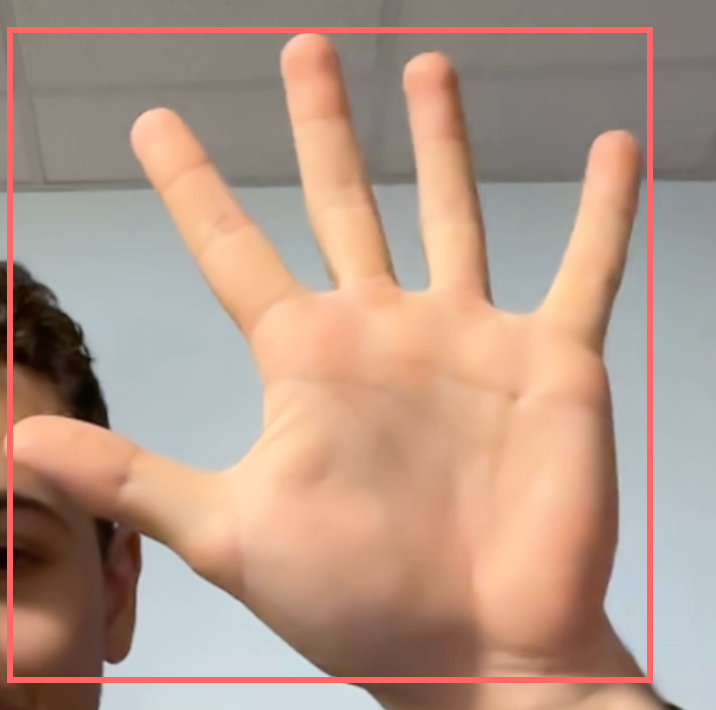
\includegraphics[width=0.5\textwidth]{images/res_attendu.png}
    \captionof{figure}{Résultat attendu}
\end{center}

\begin{minipage}{0.45\textwidth}
    \centering
    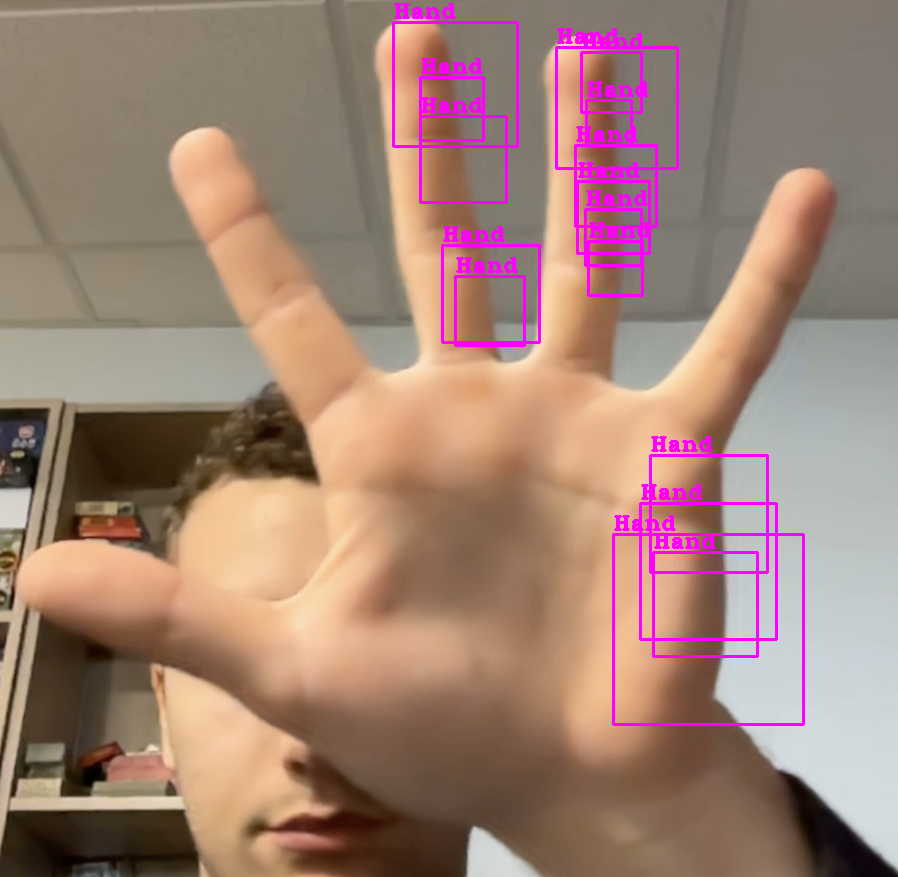
\includegraphics[width=\textwidth]{images/cascade0.png}
    \captionof{figure}{Test 1}
    \label{fig:res_cascade0}
\end{minipage}
\begin{minipage}{0.45\textwidth}
    \centering
    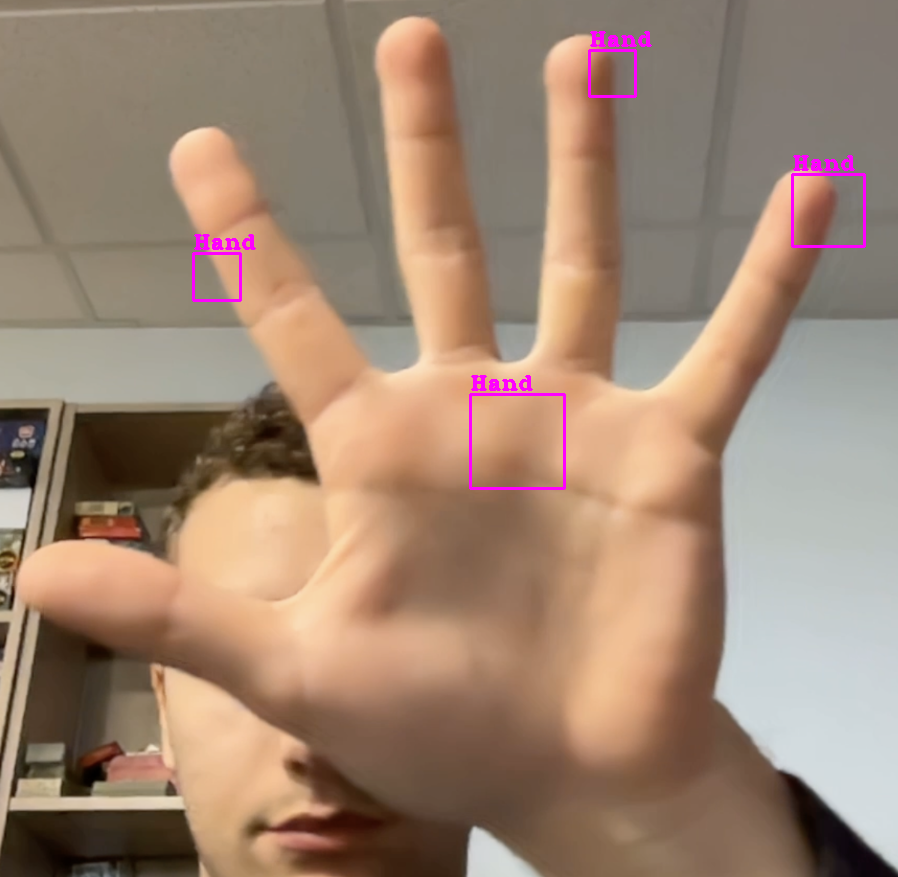
\includegraphics[width=\textwidth]{images/cascade1.png}
    \captionof{figure}{Test 2}
    \label{fig:res_cascade1}
\end{minipage}


\begin{minipage}{0.45\textwidth}
    \centering
    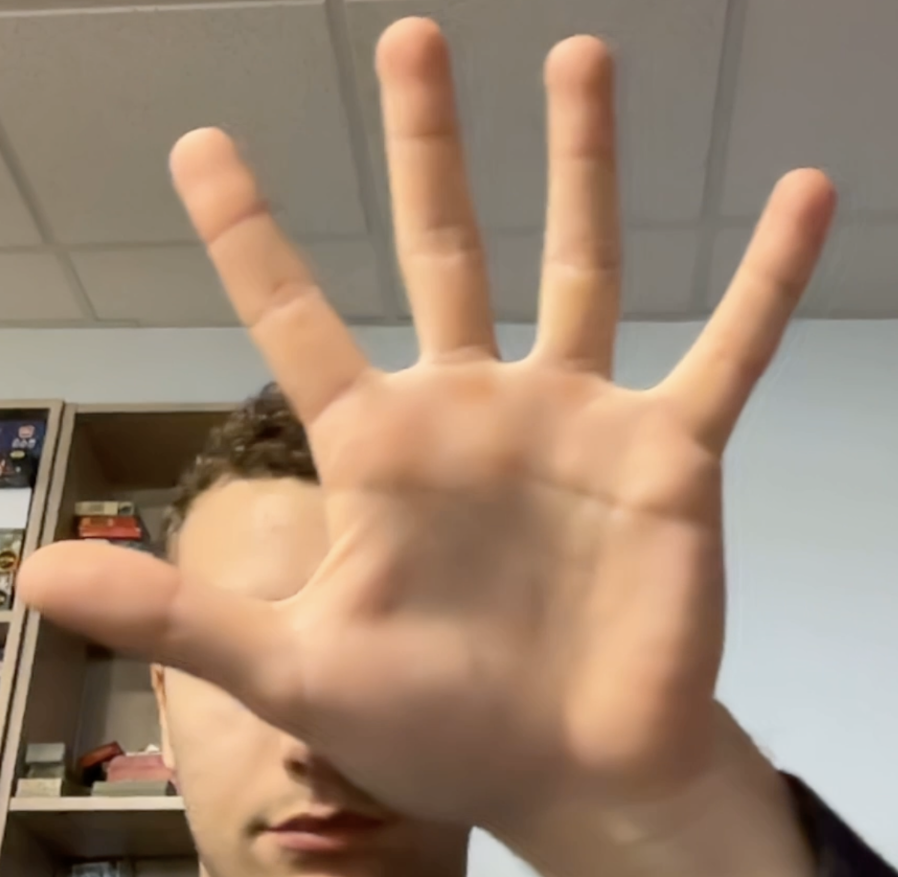
\includegraphics[width=\textwidth]{images/cascade2.png}
    \captionof{figure}{Test 3}
    \label{fig:res_cascade2}
\end{minipage}
\begin{minipage}{0.45\textwidth}
    \centering
    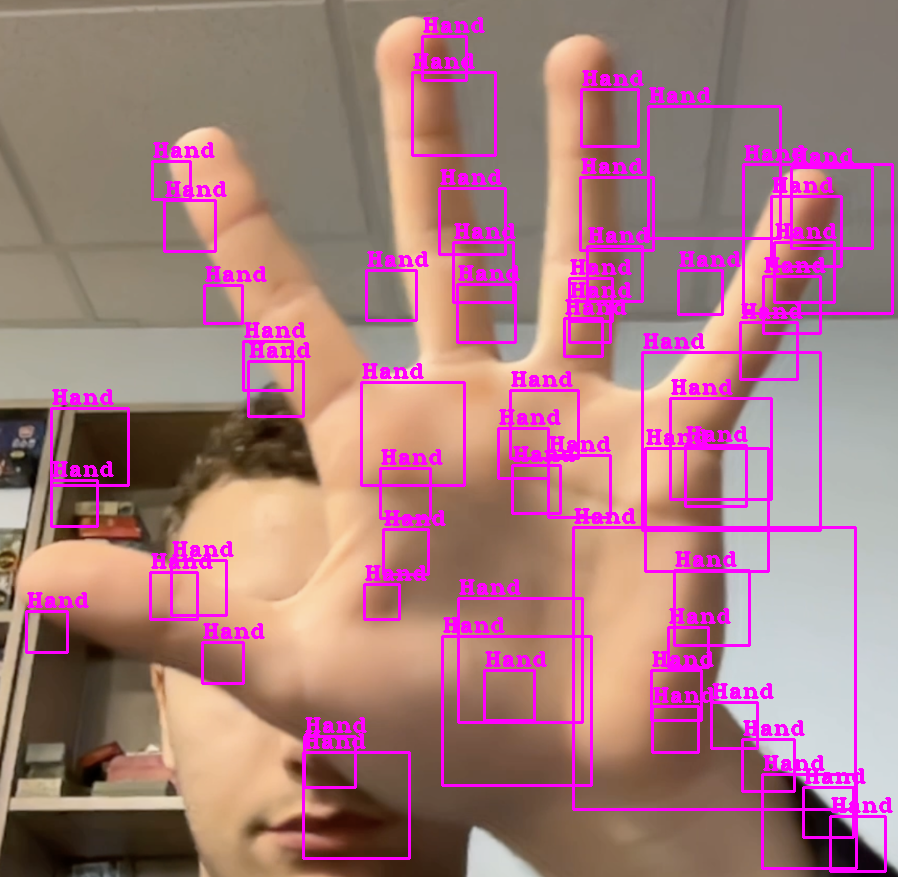
\includegraphics[width=\textwidth]{images/cascade3.png}
    \captionof{figure}{Test 4}
    \label{fig:res_cascade3}
\end{minipage}

\bigbreak

Les classifieurs 1 (Fig. \ref{fig:res_cascade0}) et 2 (Fig. \ref{fig:res_cascade1}) ne détectent pas entièrement la main dans l'image, seulement plusieurs portions plus ou moins grandes. Le classifieur 4 (Fig. \ref{fig:res_cascade3}) détecte bien la main mais détecte aussi d'autres objets dans l'image. Le classifieur 3 (Fig. \ref{fig:res_cascade2}) est le moins satisfaisant puisqu'il ne détecte rien du tout, certainement dû à un surapprentissage.

\paragraph{Conclusion}
Les résultats ne sont pas entièrement satisfaisant. En effet, les différents classifieurs, lorsqu'ils détectent la main, ne la détectent pas entièrement mais seulement plusieurs parties. Celà est certainement dû au fait que les images positives ne contienent que la main sans "background". 

\subsubsection{En créant nous même des images positives}
\paragraph{Méthodologie}
N'ayant pas obtenus de résultats satisfaisants avec la base de données d'images de mains, nous avons décidé de créer nous même des images positives. Pour cela, nous avons utilisé la librairie OpenCV pour ajouter une image de main aux images positives (Fig. \ref{fig:ex_pos_neg}). Nous avons ensuite généré les fichiers de descriptions des images positives et entrainé le classifieur à l'aide de ces fichiers. \bigbreak

\begin{center}
    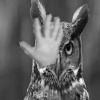
\includegraphics[width=0.5\textwidth]{images/ex_pos_neg.jpg}
    \captionof{figure}{Exemple d'image positive créée à partir d'une image négative}
    \label{fig:ex_pos_neg}
\end{center}

\noindent Comme précédemment, nous avons tester différents paramètres pour l'entrainement du classifieur. \bigbreak

\begin{center} 
    \begin{tabular}{|c|c|c|c|c|c|c|c|}
        \hline
        Test & Nombre de & Nombre de & Nombre & Profondeur & Acceptance  & Mode & Temps \\
        & positifs & négatifs & d'étapes & d'arbre & Ratio Break &  &  \\ 
        \hline 
        5 & 8 000 & 6 000 & 15 & 1 & 1.0e-5 & Défaut & 4h05 \\
        \hline
        6 & 8 000 & 6 000 & 10 & 1 & 1.0e-5 & Défaut & 1h53 \\
        \hline
        7 & 8 000 & 6 000 & 5 & 1 & 1.0e-5 & Défaut & 35min \\
        \hline
        8 & 5 000 & 8 000 & 9 & 1 & 1.0e-5 & All & 2h49 \\
        \hline
        9 & 5 000 & 8 000 & 5 & 1 & 1.0e-5 & All & 1h25 \\
        \hline
    \end{tabular}
\end{center}


\paragraph{Résultats}

\begin{minipage}{0.45\textwidth}
    \centering
    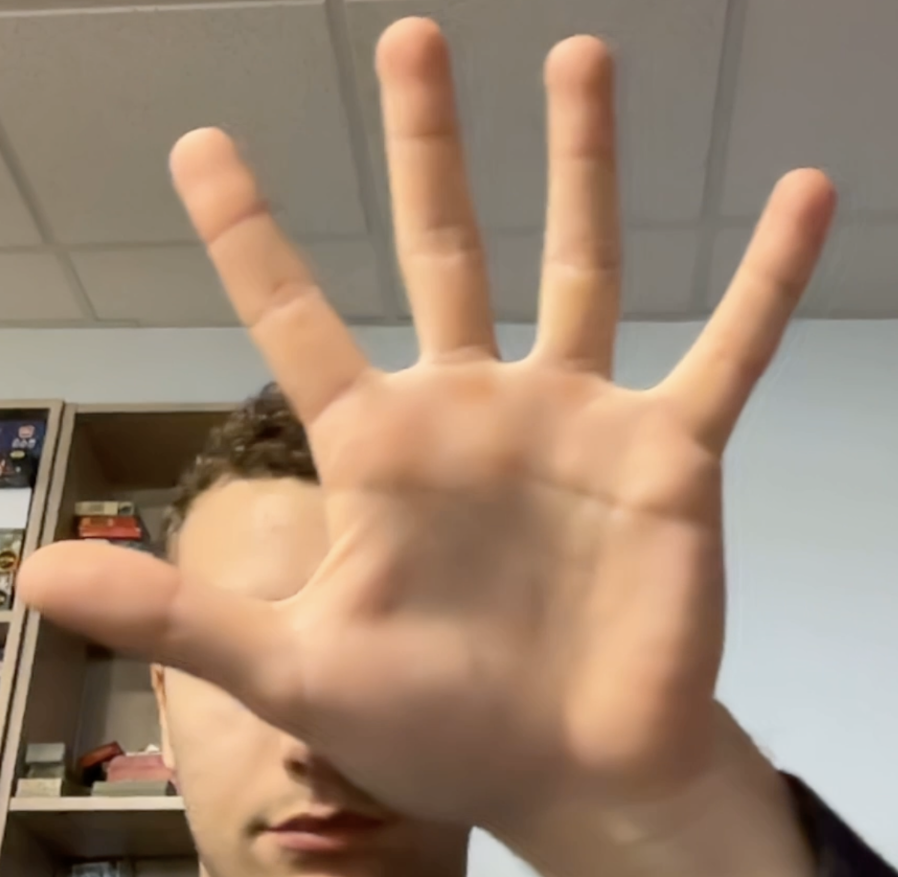
\includegraphics[width=\textwidth]{images/cascade4.png}
    \captionof{figure}{Test 5}
    \label{fig:res_cascade4}
\end{minipage}
\begin{minipage}{0.45\textwidth}
    \centering
    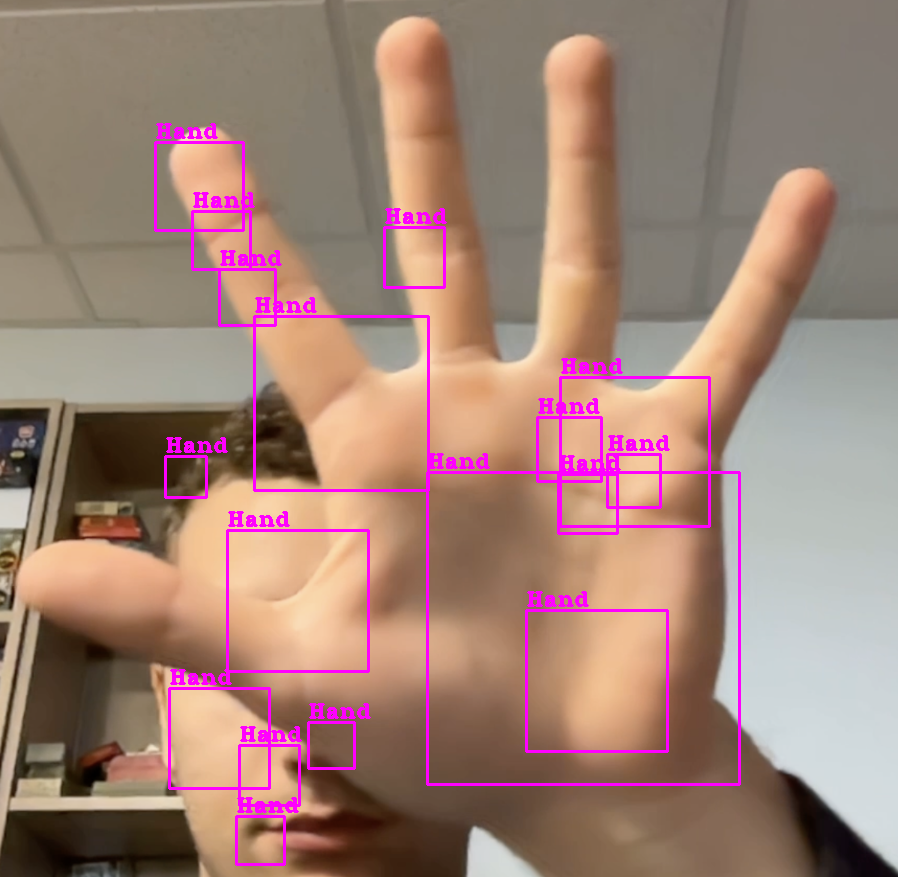
\includegraphics[width=\textwidth]{images/cascade5.png}
    \captionof{figure}{Test 6}
    \label{fig:res_cascade5}
\end{minipage}

\begin{minipage}{0.45\textwidth}
    \centering
    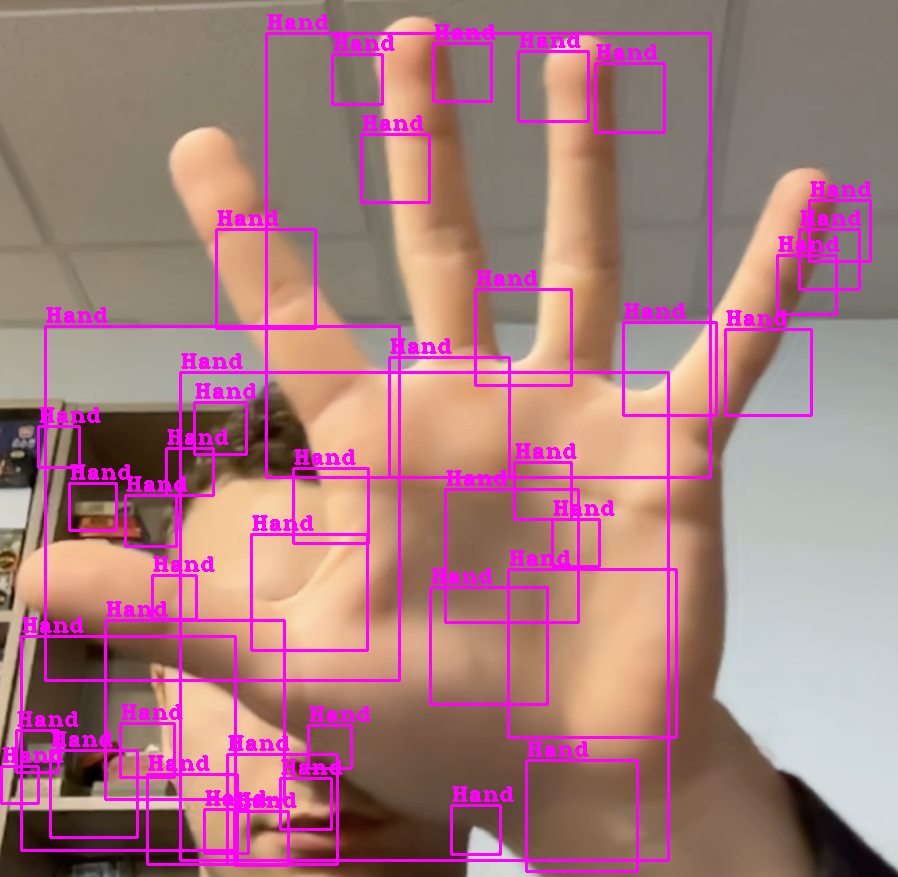
\includegraphics[width=\textwidth]{images/cascade6.png}
    \captionof{figure}{Test 7}
    \label{fig:res_cascade6}
\end{minipage}
\begin{minipage}{0.45\textwidth}
    \centering
    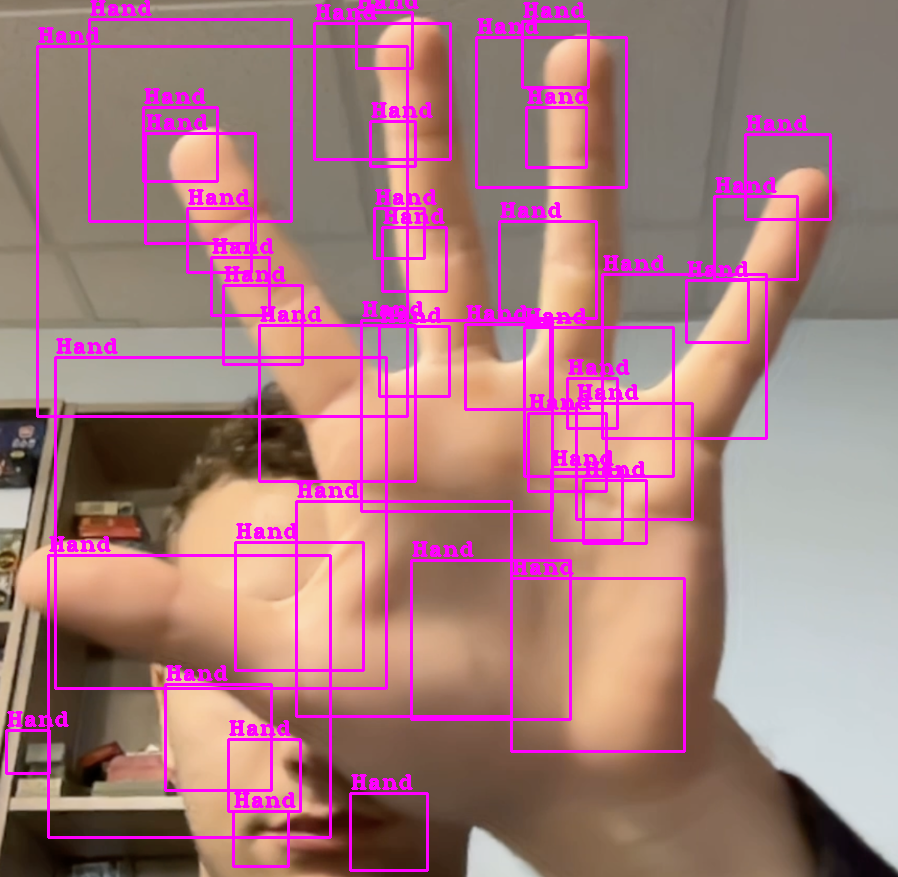
\includegraphics[width=\textwidth]{images/cascade7.png}
    \captionof{figure}{Test 8}
    \label{fig:res_cascade7}
\end{minipage}

\begin{minipage}{0.45\textwidth}
    \centering
    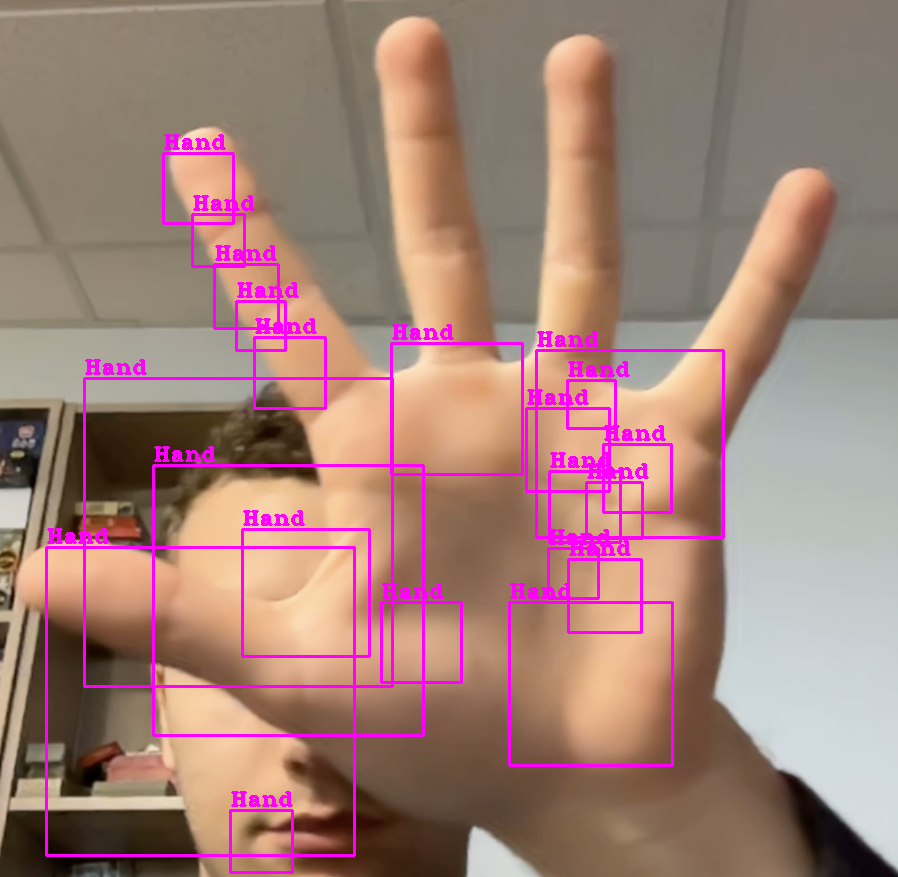
\includegraphics[width=\textwidth]{images/cascade8.png}
    \captionof{figure}{Test 9}
    \label{fig:res_cascade8}
\end{minipage}
\begin{minipage}{0.45\textwidth}
    \centering
    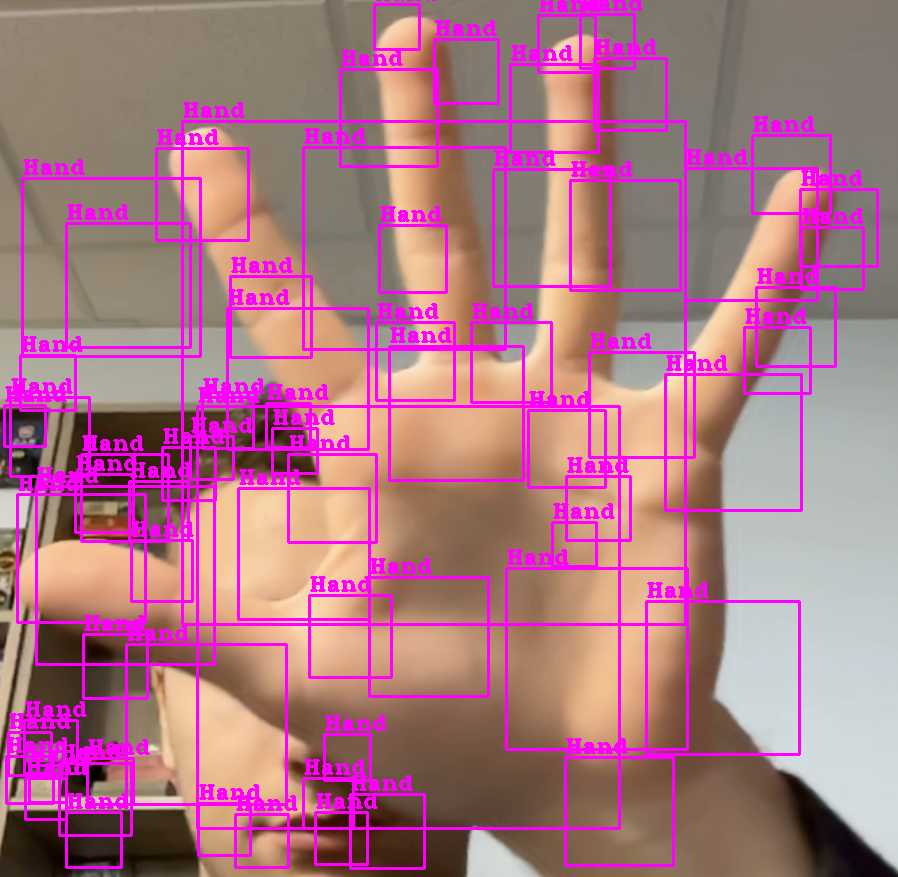
\includegraphics[width=\textwidth]{images/cascade9.png}
    \captionof{figure}{Test 10}
    \label{fig:res_cascade9}
\end{minipage}
\bigbreak

Les résultats ne sont pas satisfaisants. Le classifieur 5 (Fig. \ref{fig:res_cascade4}) ne détecte rien du tout, certainement dû à un surapprentissage. Les classifieurs 7 (Fig. \ref{fig:res_cascade6}), 8 (Fig. \ref{fig:res_cascade7}) et 10 (Fig. \ref{fig:res_cascade9}) détectent bien la main mais détectent aussi beaucoup d'autres objets dans l'image. Les classifieurs 6 (Fig. \ref{fig:res_cascade5}) et 9 (Fig. \ref{fig:res_cascade8}) ne détectent pas entièrement la main dans l'image, seulement plusieurs portions plus ou moins grandes. Ils détectent aussi notamment une partie de la bouche. 

\paragraph{Conclusion}
Les résultats ne sont pas beaucoup plus satisfaisant. On obtient dans l'ensemble,les mêmes résultats que précédemment c'est-à-dire des détections partiels de la main et non la main entières pour les classifieurs les mieux entrainés.

Il faudrait essayer de prendre une base de données de mains contenant des background différents et annoter nous mêmes les images, c'est-à-dire l'emplacement des mains dans l'image, pour voir si celà améliore les résultats. 

\section{Reconnaissance de la main par traitement d'image}
\subsection{Méthodologie}
Pour réussir à détecter la main sans classifieur, nous avons dû tester plusieurs méthodes. En effet, plusieurs paramètres interviennent afin d'avoir une détection de la main optimale.
Nous avons dû jouer sur plusieurs paramètres :
\begin{itemize}[label=-]
    \item Le format de la couleur de l'image : GreyScale ou HSV
    \item Flou : avec ou sans, quel type de flou (Gaussien ou Bilatéral)
    \item Thresholding : pour binariser l'image. Il y avait là plusieurs paramètres possibles : le seuil et le type de thresholding (binaire, binaire inversé, tronqué, to zero, to zero inversé)
    \item Contours : pour détecter les contours de la main. Là aussi, plusieurs paramètres possibles.
\end{itemize}

\subsection{Expériences et résultats}
Pour trouver les meilleures paramètres, nous avons testé plusieurs combinaisons de paramètres, avec ou sans flou, avec ou sans Canny ...

\bigbreak

Tout d'abord, nous avons essayé en essayant de mettre l'images en gris, puis de flouter l'image avec un flou gaussien, puis de binariser l'image avec un thresholding binaire. Enfin, nous avons utilisé Canny pour détecter les contours de la main et nous avons tracer le convex hull de la main. Les résultats sont plutôt bons puisque nous avons capturé l'essentiel de la main même si il manque une grosse partie du pouce.\bigbreak

\begin{center}
    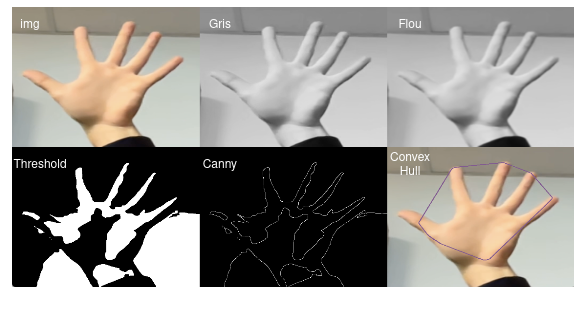
\includegraphics[width=\textwidth]{images/pre_ttt_1.png}
    \captionof{figure}{Résultat de la détection de la main : Thresholding : seuil entre 200-255, TRESH\_BINARY, Contours : RETR\_EXTERNAL, CHAIN\_APPROX\_SIMPLE}
\end{center}
\bigbreak

\bigbreak

Nous avons aussi essayé sans flou, les résultats étaient moins bons puisque nous pouvons voir plusieurs convex hulls pour une seule main. 
\bigbreak

\begin{center}
    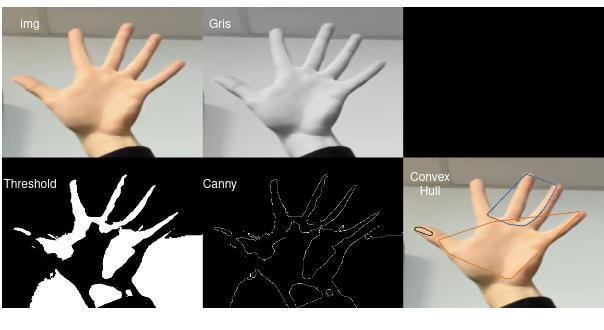
\includegraphics[width=\textwidth]{images/pre_ttt_2.png}
    \captionof{figure}{Résultat de la détection de la main : Thresholding : seuil entre 198-255, TRESH\_BINARY, Contours : RETR\_EXTERNAL, CHAIN\_APPROX\_SIMPLE}
\end{center}
\bigbreak

Nous avons ensuite essayé sans flou et sans Canny. Les résultats sont encores moins bons puisque nous avons plusieurs convex hulls voir même certains hors de la main. \bigbreak

\begin{center}
    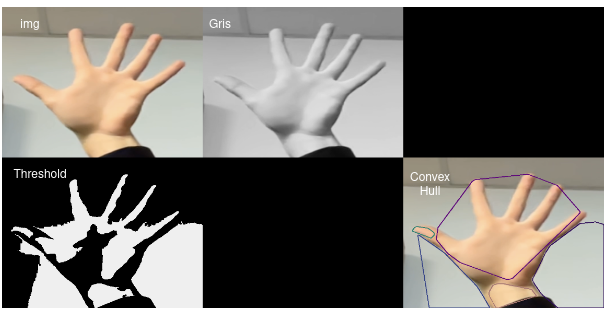
\includegraphics[width=\textwidth]{images/pre_ttt_3.png}
    \captionof{figure}{Résultat de la détection de la main : Thresholding : seuil entre 196-239, TRESH\_BINARY, Contours : RETR\_EXTERNAL, CHAIN\_APPROX\_SIMPLE}
\end{center}
\bigbreak

Les résultats ne sont pas exceptionnels mais nous nous attendions à ce qu'ils soient meilleurs en passant l'image en HSV plutôt qu'en GreyScale.  \bigbreak

\begin{center}
    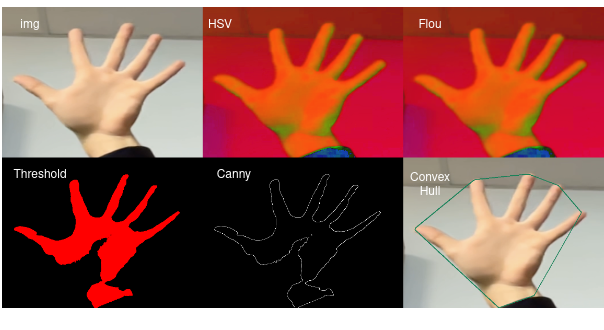
\includegraphics[width=\textwidth]{images/pre_ttt_4.png}
    \captionof{figure}{Résultat de la détection de la main : Thresholding : seuil entre 223-255, TRESH\_BINARY, Contours : RETR\_EXTERNAL, CHAIN\_APPROX\_SIMPLE}
\end{center}
\bigbreak

On voit clairement ici que les résultats sont meilleurs puisque nous avons bien capturé l'ensemble de la main. De plus, même sur une image de mauvaise qualité, en jouant sur les paramètres, nous avons réussi à capturer la main. \bigbreak

\begin{center}
    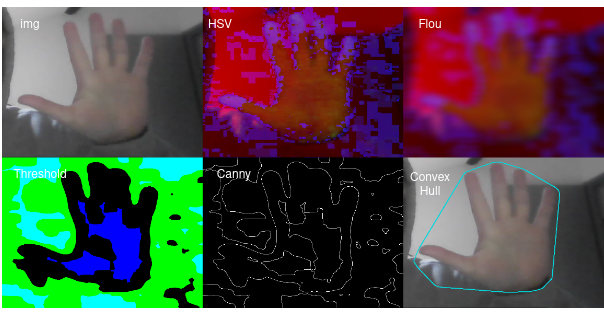
\includegraphics[width=\textwidth]{images/pre_ttt_5.png}
    \captionof{figure}{Résultat de la détection de la main : Flou : X = 41, Y = 27, Sigma = 22 ; Thresholding : seuil entre 11-255, TRESH\_BINARY ; Contours : RETR\_EXTERNAL, CHAIN\_APPROX\_SIMPLE}
    \end{center}
\bigbreak

Enfin, nous avons essayé sans passer par les fonctions thresholding et canny d'OpenCV mais en créant nous même un masque en fonction de la saturation, de la valeur et de la teinte. \bigbreak

\begin{center}
    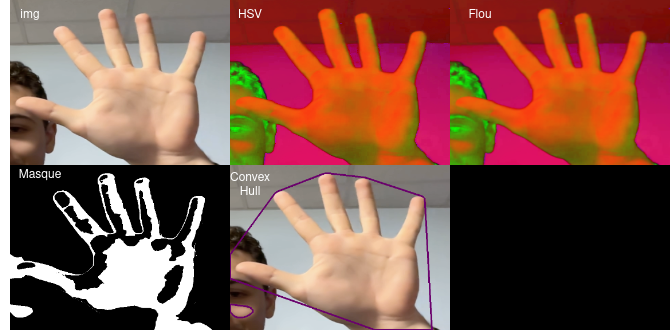
\includegraphics[width=\textwidth]{images/pre_ttt_6.png}
    \captionof{figure}{Résultat de la détection de la main : Hue : 0 - 94, Saturation : 37 - 180, Value : 145 - 238}
\end{center}
\bigbreak

Les résultats obtenus sont bons. Nous arrivons bien a détecter la main. Cependant, ces résultats sont très dépendant des valeurs des paramètres. 

\subsection{Conclusion}
Même si les résultats en passant l'image en HSV sont concluants, il reste encore des améliorations à apporter puisque la détection est très dépendante des paramètres utilisés. Il faudrait donc trouver une méthode pour que le programme puisse trouver les meilleurs paramètres pour la détection de la main. 


\section{Fusion des deux méthodes}
\subsection{Méthodologie}
Nous avons un classifieur d'une part qui détecte une portion de la main et d'autres part un système qui permet de détecter la main si les paramètres sont biens configurés. Nous avons donc essayer de fusionner ces deux méthodes pour avoir une meilleure détection de la main. 

\begin{center}
    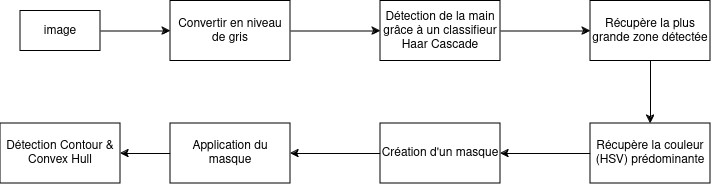
\includegraphics[width=\textwidth]{images/pipeline_combinaison.png}
    \captionof{figure}{Pipeline de la fusion des deux méthodes}
    \label{fig:pipeline_combinaison}
\end{center}

La méthodologie est la suivante (Fig. \ref{fig:pipeline_combinaison}) : à partir d'un image que nous convertissons en niveau de gris, nous essayons de détecter la main grâce à un classifieur Haar-cascade. Nos classifieurs détectant plusieurs zone au niveau de la main, nous récupérons la plus grosse. Nous passons ensuite cette zone en HSV afin de récupéré la teinte, saturation et valeur majoritaire de la zone. Nous créons ensuite un masque en fonction de ces valeurs et d'un epsilon afin d'avoir un seuil minimum et un seuil maximum. Nous passons ensuite ce masque sur l'image et affichons le Convex Hull correspondant.  

\subsection{Expériences et résultats}


\begin{center}
    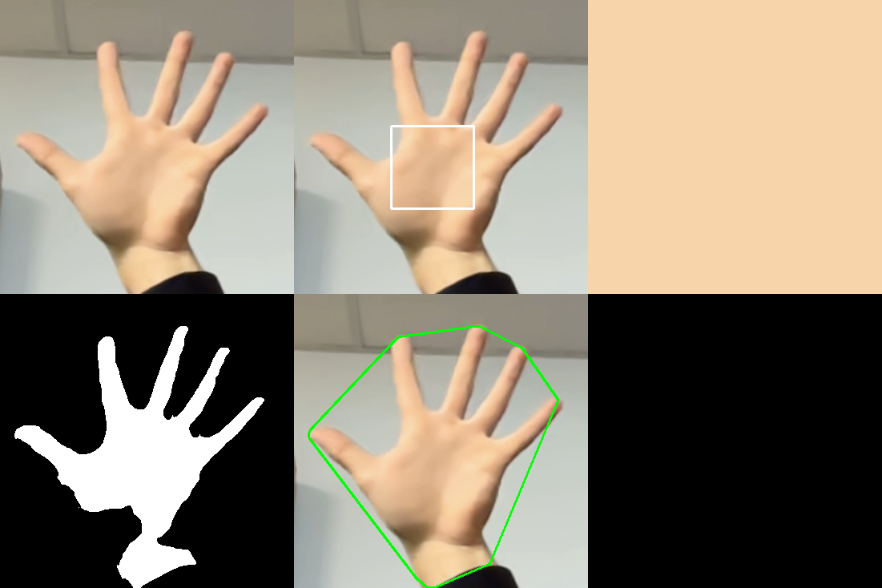
\includegraphics[width=\textwidth]{images/res_combinaison_5_doigts.png}
    \captionof{figure}{Résultat de la fusion des deux méthodes.}
    \label{fig:res_combinaison_5_doigts}
\end{center}

Nous pouvons voir (Fig. \ref{fig:res_combinaison_5_doigts}) que la fusion des deux méthodes fonctionne bien. Nous avons bien détecté la main et les 5 doigts. \bigbreak

Cependant, cette méthode ne fonctionne ne semble fonctionner qu'avec une main ouverte et 5 doigts levés. \bigbreak

\begin{center}
    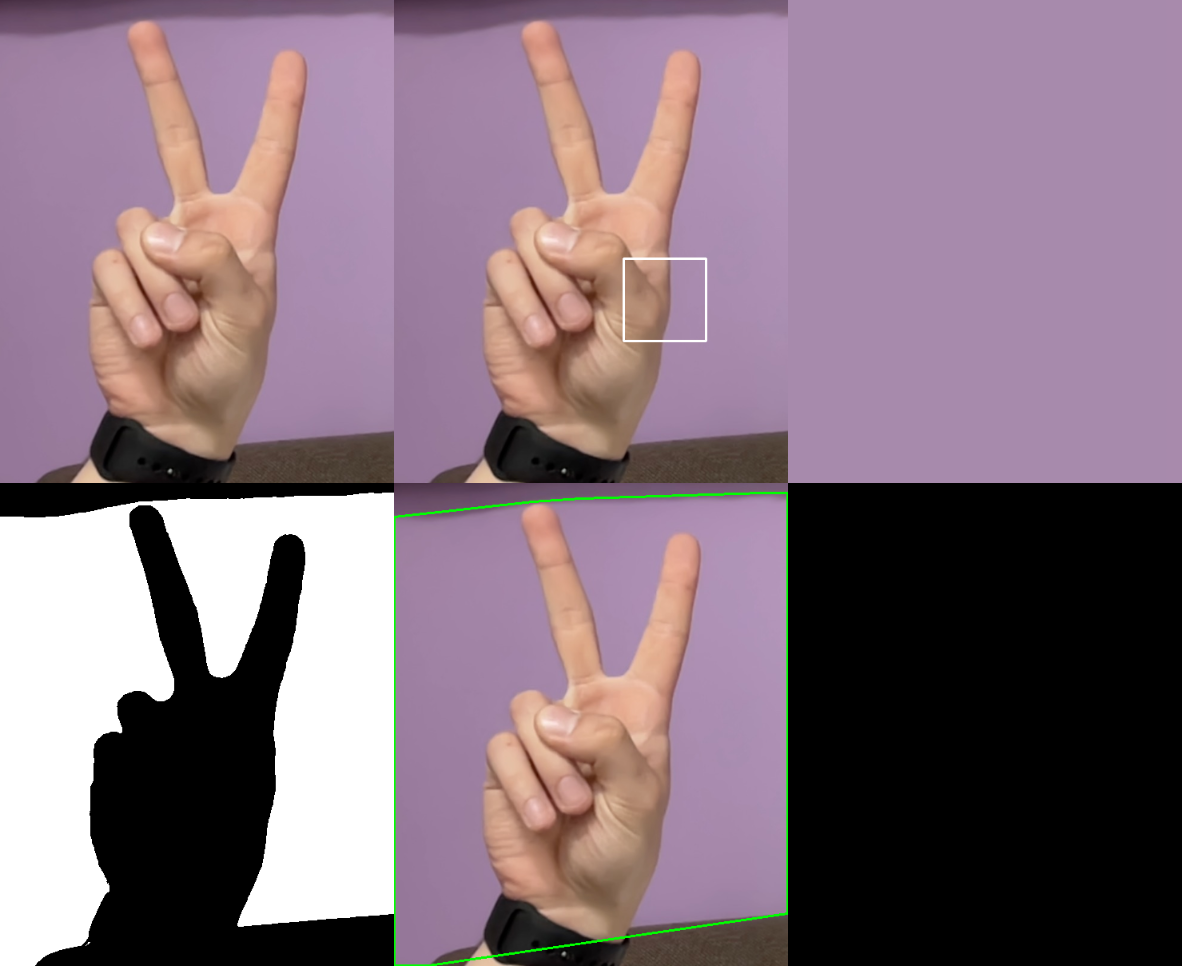
\includegraphics[width=\textwidth]{images/res_combinaison_2_doigts.png}
    \captionof{figure}{Résultat de la fusion des deux méthodes avec 2 doigts levé.}
    \label{fig:res_combinaison_2_doigts}
\end{center}

En effet, lorsque nous avons ensuite essayé avec 2 doigts levés (Fig. \ref{fig:res_combinaison_2_doigts}), une partie de la main est bien détecté. Cependant, étant donné que nous récupérons la couleur majoritaire de la zone détecté, nous avons ici la couleur du fond de l'image et non de la main car même si la zone représentant une partie de la main semble être légèrement plus grande, les nuances de couleurs y sont aussi beaucoup plus nombreuses. 

\subsection{Conclusion}
Cette méthode rencontre deux problèmes principaux. Tout d'abord, elle fonctionne beaucoup mieux sur une main ouverte avec 5 doigts levés car le classifieur a été entrainé pour reconnaitre une main ouverte. 
De plus, récupéré la couleur majoritaire de la zone détectée ne semble pas être la meilleure méthode pour récupérer la couleur de la main. En effet, comme nous avons pu le voir précédemment, les variations dû à la luminosité ou à la qualité de l'image peuvent faire en sorte que la couleur majoritaire ne soit pas la couleur de la main. Enfin, afin d'avoir une meilleure détection, nous utilisons un paramètre "epsilon" qui permet d'avoir une plage de données plus ou moins grande pour la teinte, la saturation et la valeur. Cependant, ce paramètre peut être problèmatique car il dépend de la qualité de l'image. \bigbreak

\bigbreak


\newpage

\section{Détection des mouvements de la main}
\'Etant donné que la fusion des deux méthodes ne fonctionne pas pour tous les cas, nous avons décidé de repartir sur une méthode où nous pouvons modifier les valeurs des paramètres pour la détection de la main.

\subsection{Sans Convex Hull}

\subsubsection{Méthodologie}
Nous avons une image que nous passons en HSV à laquelle on ajoute un Flou Gaussien. Avec un système de trackbars nous ajustons ensuite les valeurs minimales et maximales pour la teinte, la luminosité et la valeur afin d'avoir un masque qui ne détecte que la main. Nous passons ensuite ce masque sur l'image et détectons les contours de la main. Pour la détection des doigts, nous avons ensuite créer différents masques que nous passons ensuite sur l'image. Nous déplaçons ensuite ce masque sur l'image et calculons le nombre de pixels blancs dans le masque. Si ce nombre est entre un certains seuil, alors nous considérons que le doigt est présent. \bigbreak

\begin{center}
    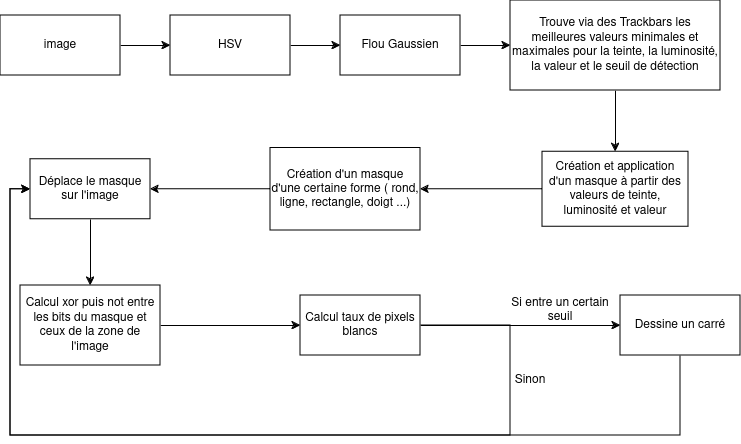
\includegraphics[width=\textwidth]{images/pipeline_detect_fingers_sans_convex_hull.png}
    \captionof{figure}{Pipeline de la détection des doigts sans Convex Hull}
    \label{fig:pipeline_detect_fingers_sans_convex_hull}
\end{center}

\subsubsection{Expériences et résultats}

{\LARGE TO DO}
\begin{center}
    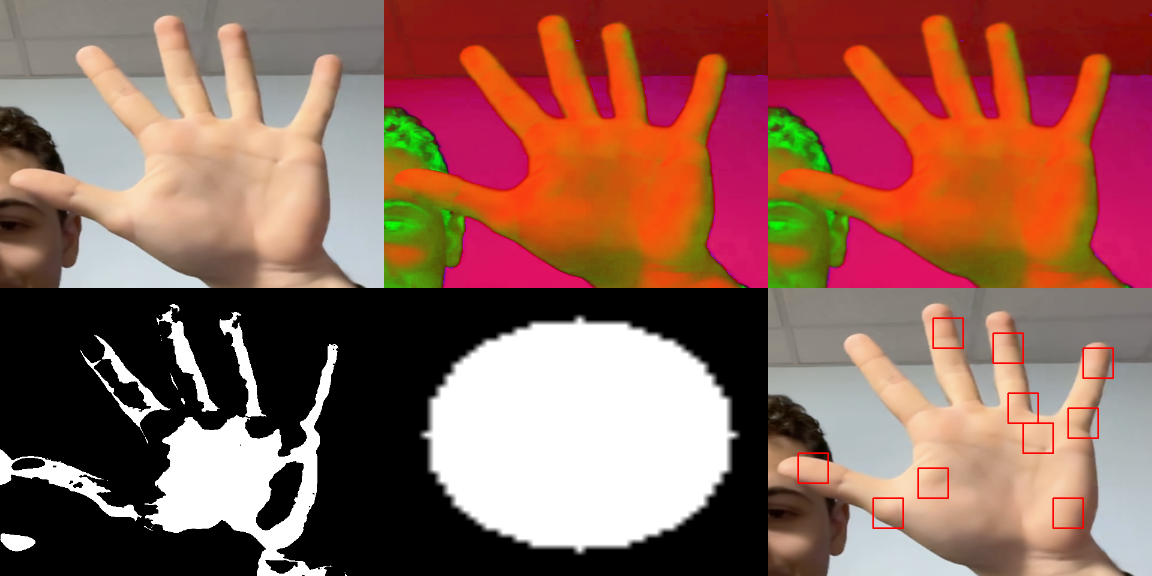
\includegraphics[width=\textwidth]{images/detect_fingers_mask_4.png}
    \captionof{figure}{Détection des doigts sans Convex Hull. Teinte : 10 - 43 ; Saturation : 79 - 150 ; Valeur : 174 - 237 ; Seuil : 65 - 75}
    \label{fig:detect_fingers_mask_4}
\end{center}

\begin{center}
    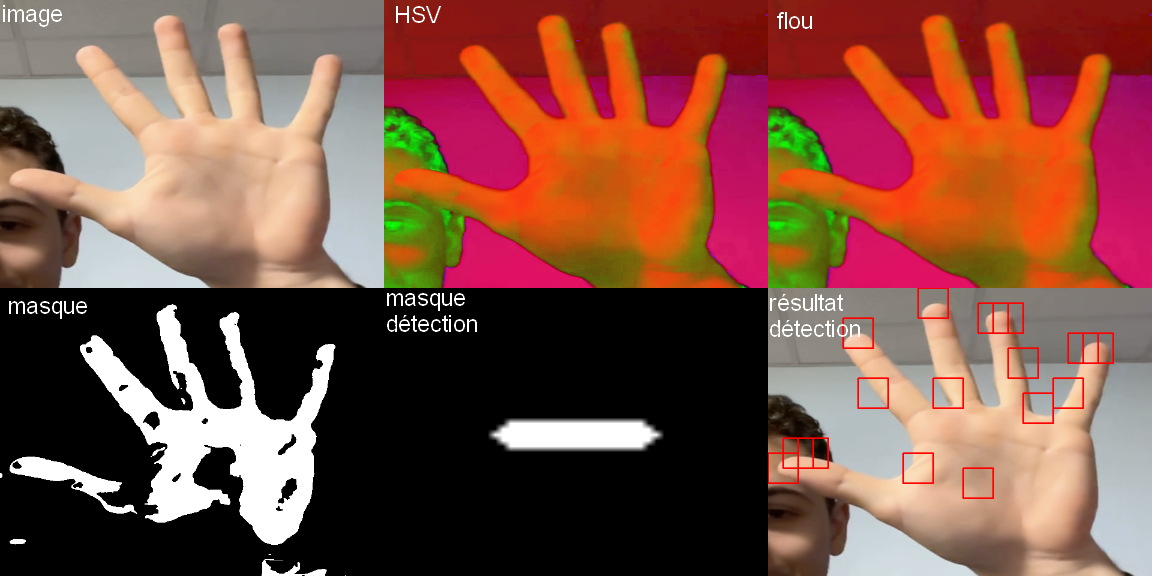
\includegraphics[width=\textwidth]{images/detect_fingers_mask_5.png}
    \captionof{figure}{Détection des doigts sans Convex Hull. Teinte : 9 - 41 ; Saturation : 79 - 150 ; Valeur : 202 - 255 ; Seuil : 62 - 75}
    \label{fig:detect_fingers_mask_5}
\end{center}

\begin{center}
    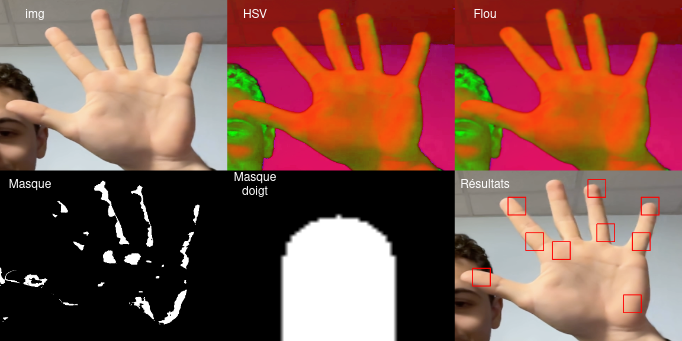
\includegraphics[width=\textwidth]{images/detect_fingers.png}
    \captionof{figure}{Détection des doigts sans Convex Hull. Teinte : 8 - 67 ; Saturation : 97 - 128 ; Valeur : 185 - 239 ; Seuil : 73 - 100}
    \label{fig:detect_fingers}
\end{center}


\begin{center}
    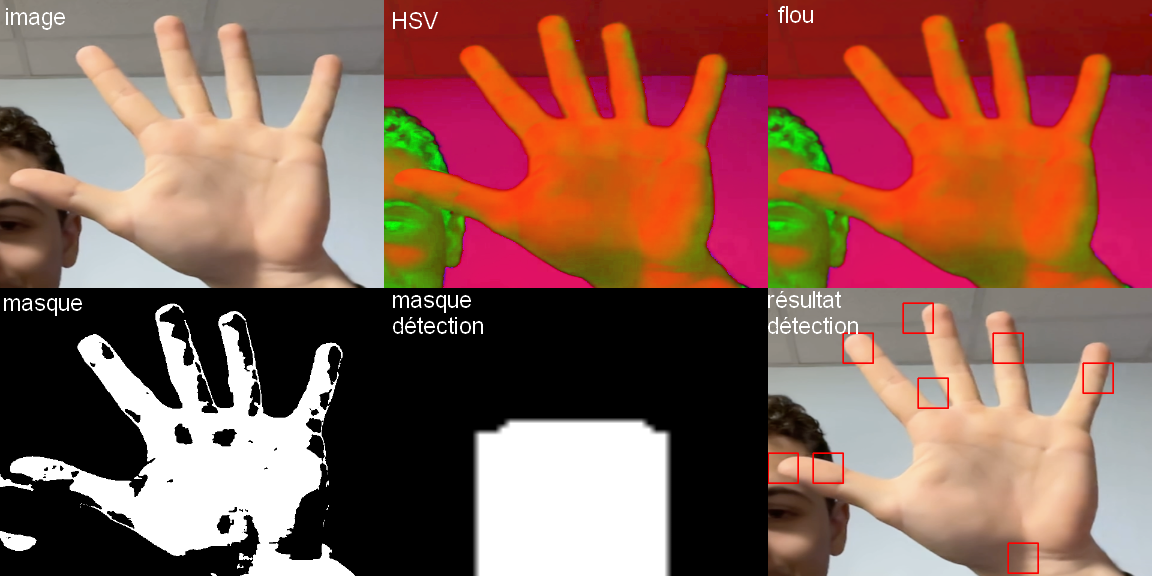
\includegraphics[width=\textwidth]{images/detect_fingers_mask_2.png}
    \captionof{figure}{Détection des doigts sans Convex Hull. Teinte : 8 - 59 ; Saturation : 66 - 98 ; Valeur : 112 - 255 ; Seuil : 54 - 57}
    \label{fig:detect_fingers_mask_2}
\end{center}

\begin{center}
    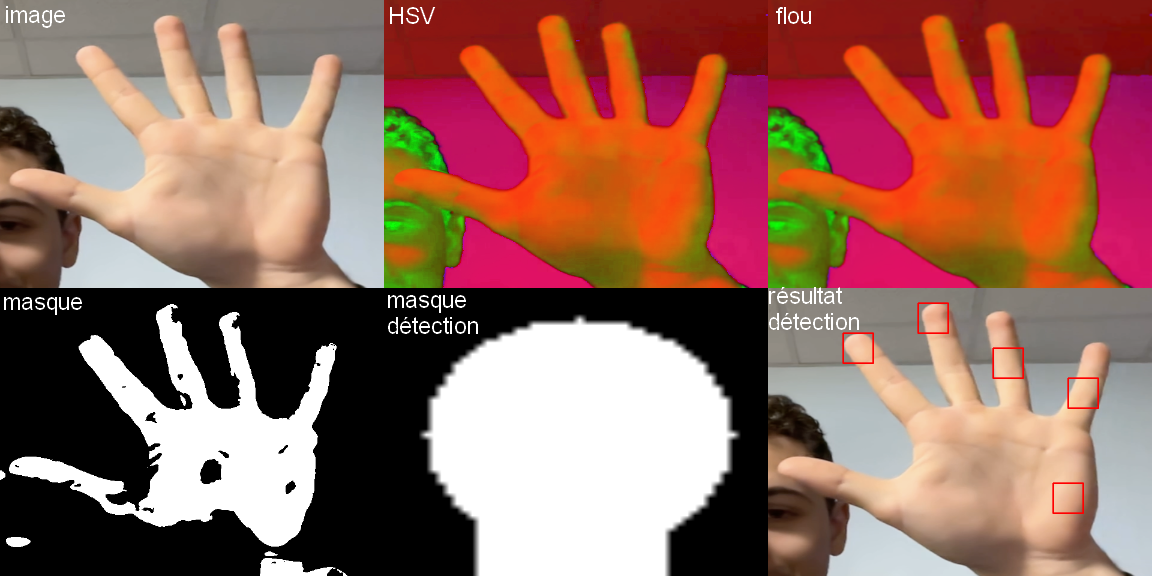
\includegraphics[width=\textwidth]{images/detect_fingers_mask_3.png}
    \captionof{figure}{Détection des doigts sans Convex Hull. Teinte : 10 - 72 ; Saturation : 75 - 147 ; Valeur : 193 - 255 ; Seuil : 71 - 100}
    \label{fig:detect_fingers_mask_3}
\end{center}

\newpage


\subsection{Avec Convex Hull}
\subsubsection{Méthodologie}
Le début est le même que précédemment. Nous avons une image que nous passons en HSV à laquelle on ajoute un Flou Gaussien. Avec un système de trackbars nous ajustons ensuite les valeurs minimales et maximales pour la teinte, la luminosité et la valeur afin d'avoir un masque qui ne détecte que la main. Nous passons ensuite ce masque sur l'image et détectons les contours de la main. Nous utilisons ensuite la fonction Convex Hull d'OpenCV pour tracer le contour de la main. Nous récupérons ensuite les points du Convex Hull et les affichons sur l'image. Nous créons ensuite des filtres afin de n'avoir seulement les points qui nous intérésse. \bigbreak

\begin{center}
    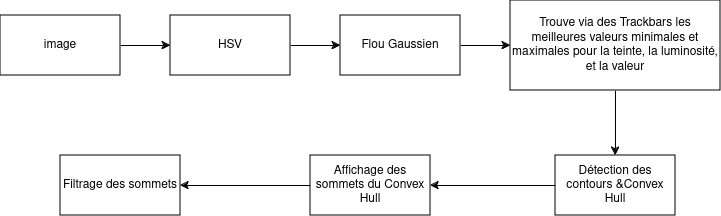
\includegraphics[width=\textwidth]{images/pipeline_detect_fingers_avec_convex_hull.png}
    \captionof{figure}{Pipeline de la détection des doigts avec Convex Hull}
    \label{fig:pipeline_detect_fingers_avec_convex_hull}
\end{center}

\subsubsection{Résultats}

\begin{center}
    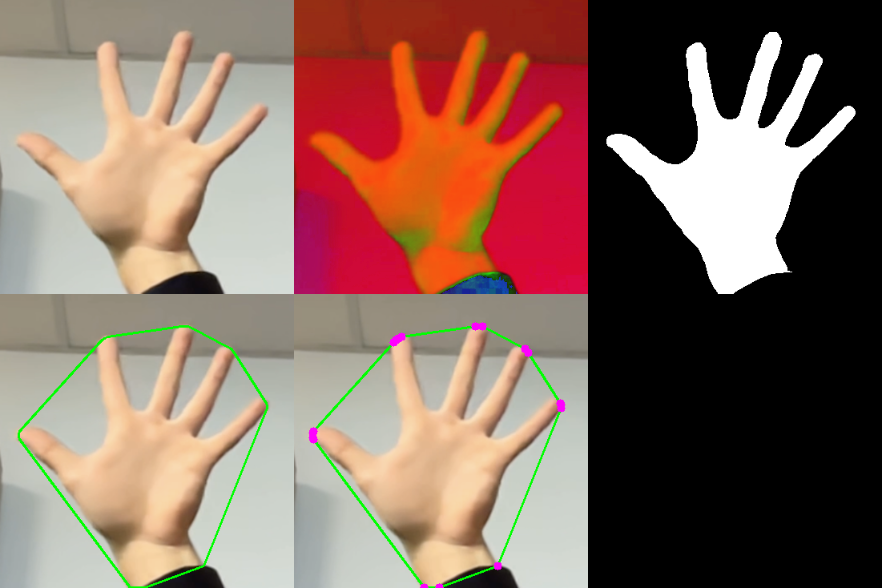
\includegraphics[width=\textwidth]{images/res_5_convex_hull_no_filter_pt.png}
    \captionof{figure}{Résultat obtenus avec Convex Hull}
    \label{fig:res_5_convex_hull_no_filter_pt}
\end{center}

Comme nous pouvons le voir (Fig. \ref{fig:res_5_convex_hull_no_filter_pt}), la détection des doigts est plutôt bonne. Nous avons bien des petits cercles qui apparaissent au bout des doigts. Cependant, étant donné que nous affichons les sommets du Convex Hull, nous avons plusieurs points au bout de chaque doigts ainsi qu'en bas de la main. \bigbreak

Nous avons donc essayé de filtrer les points : tout d'abord au niveau des doigts nous gardons un seul point par doigt. Ensuite, nous filtrons les points en bas de la main : si la coordonnée y d'un point est 1.5 fois inférieur à la moyenne des coordonnées y des points, alors nous le supprimons. \bigbreak

\begin{center}
    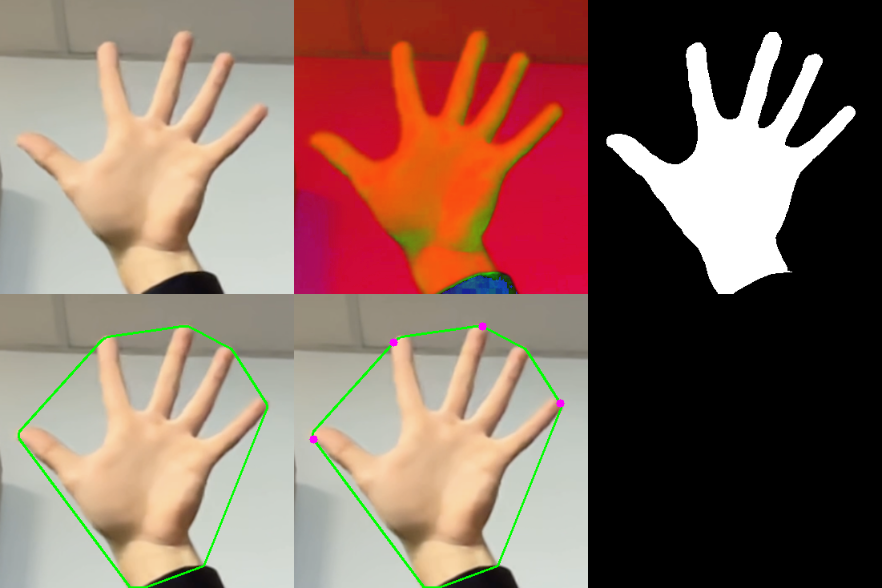
\includegraphics[width=\textwidth]{images/res_5_convex_hull_filter_1_y.png}
    \captionof{figure}{Résultat obtenus avec Convex Hull et filtrage des points}
    \label{fig:res_5_convex_hull_filter_1_y}
\end{center}

Les résultats sont meilleurs (Fig. \ref{fig:res_5_convex_hull_filter_1_y}). Nous avons bien un seul point par doigt et les points en bas de la main ont été supprimés. \bigbreak

Nous avons donc ensuite essayé sur d'autres images avec moins de doigts levés. \bigbreak

\begin{center}
    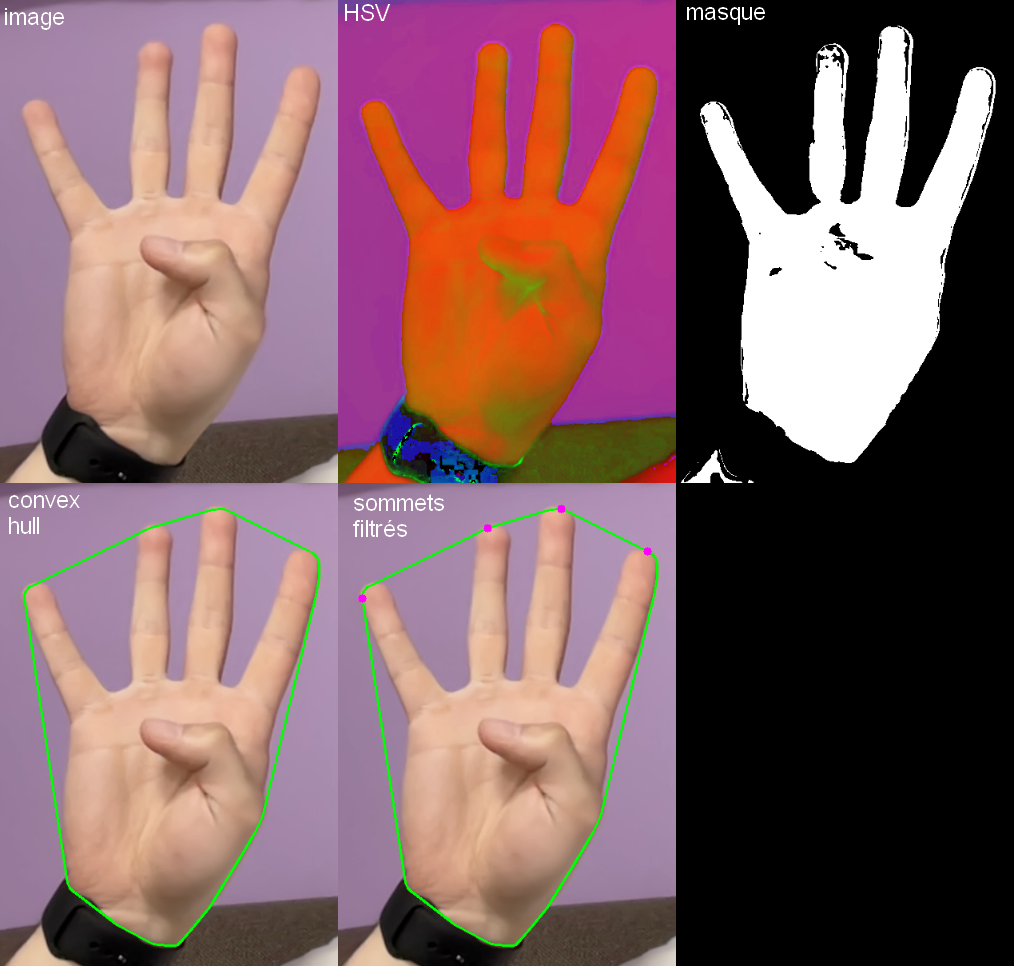
\includegraphics[width=\textwidth]{images/res_4_convex_hull_filter_1_y.png}
    \captionof{figure}{Résultat obtenus avec Convex Hull et filtrage des points}
    \label{fig:res_4_convex_hull_filter_1_y}
\end{center}

Les résultats (Fig. \ref{fig:res_4_convex_hull_filter_1_y}) sont bons avec 4 doigts, nous avons bien seulement 4 points au bout de chaque doigts.
Lorsque nous sommes passés à 3 doigts cependant, celà marchait moins bien. \bigbreak

\begin{center}
    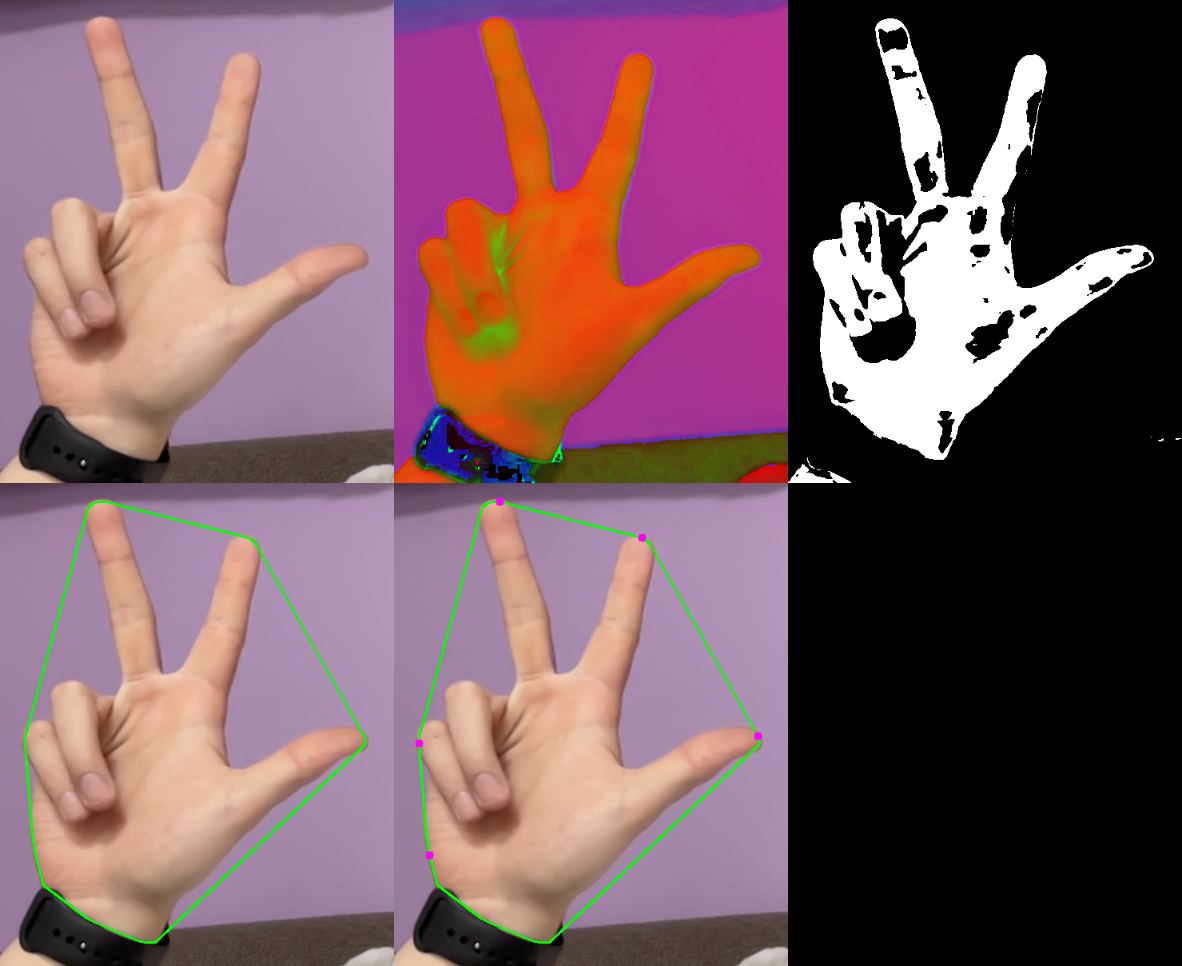
\includegraphics[width=\textwidth]{images/res_3_convex_hull_filter_1_y.png}
    \captionof{figure}{Résultat obtenus avec Convex Hull et filtrage des points}
    \label{fig:res_3_convex_hull_filter_1_y}
\end{center}

En effet, comme nous pouvons le voir nous avons 2 points à gauche qui ne sont pas des doigts et qui n'ont pas été filtré. \'Etant donné que ces points étaient l'un au dessus de l'autre nous nous sommes dis que nous pouvons les filtrer en fonction de leur coordonnées x : si la coordonnée x est quasiment la même pour deux points, alors nous les supprimons. \bigbreak

\begin{center}
    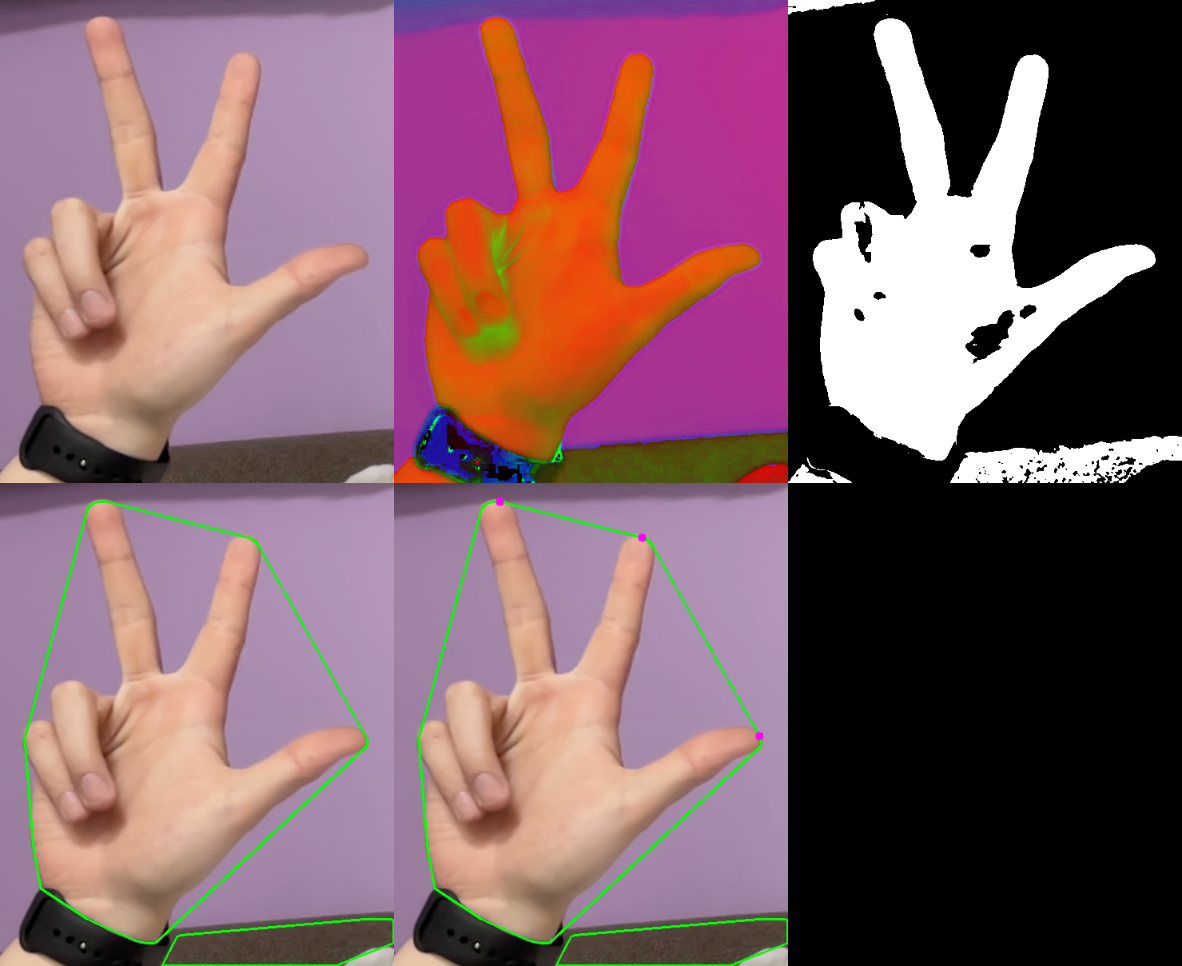
\includegraphics[width=\textwidth]{images/res_3_convex_hull_filter_1_y_1_x.png}
    \captionof{figure}{Résultat obtenus avec Convex Hull et filtrage des points}
    \label{fig:res_3_convex_hull_filter_1_y_1_x}
\end{center}

Les résultats (Fig. \ref{fig:res_3_convex_hull_filter_1_y_1_x}) sont meilleurs. Nous avons bien seulement 3 points au bout de chaque doigts. \bigbreak

Nous sommes donc passés ensuite à 2 doigts :
\begin{center}
    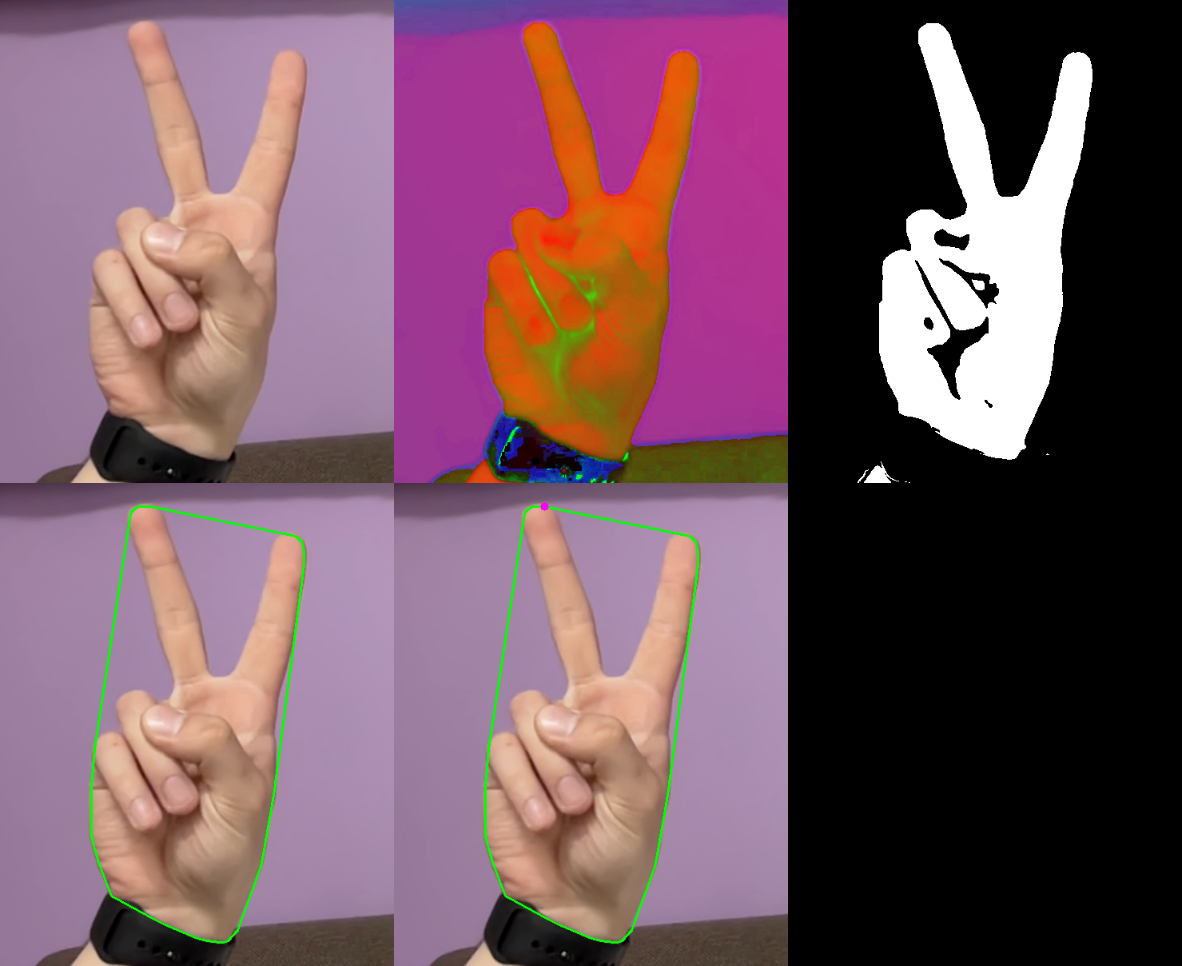
\includegraphics[width=\textwidth]{images/res_2_convex_hull_filter_1_y_1_x.png}
    \captionof{figure}{Résultat obtenus avec Convex Hull et filtrage des points}
    \label{fig:res_2_convex_hull_filter_1_y_1_x}
\end{center}

Cependant, les résultats (Fig. \ref{fig:res_2_convex_hull_filter_1_y_1_x}) ne sont pas bons. Nous avons seulement un seul cercle au lieu de deux. Lorsque nous avons regardé de plus près le problème, nous nous sommes rendus compte que le cercle au niveau de l'index était supprimé car il y avait plusieurs points juste en dessous (Fig. \ref{fig:res_2_convex_hull_all_pt}).  \bigbreak

\begin{center}
    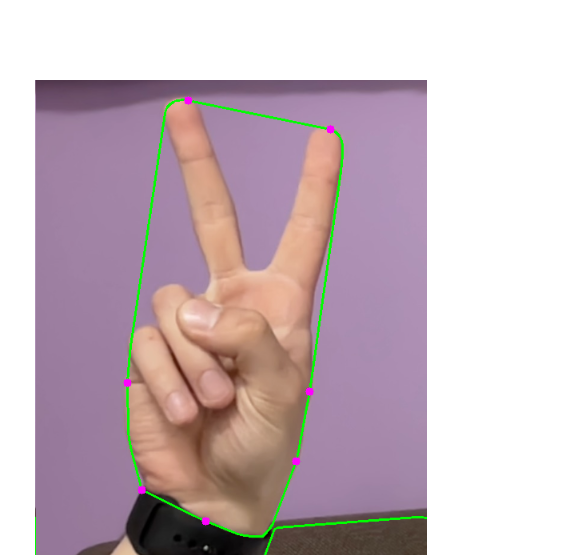
\includegraphics[width=0.5\textwidth]{images/res_2_convex_hull_all_pt.png}
    \captionof{figure}{Résultat obtenus avec Convex Hull et tous les points des sommets}
    \label{fig:res_2_convex_hull_all_pt}
\end{center}

Le point au niveau de l'index est donc supprimé car il y en a deux en dessous de lui qui sont quasiment sur la même ligne. Nous avons donc décidé de filtrer autrement : au lieu de supprimer tous les points qui sont quasiment sur la même vertical, nous avons décidé de pondéré les points en fonction de leur coordonnées en y. Le point le plus haut aura un poids de 1, le point le plus bas un poids de 0. Pour tous les points qui sont du coup sur une même vertical, nous regardons lequel est le plus grand et si le poids du plus grand est supérieur à 0.8 (donc si il est proche du haut), alors nous le gardons. \bigbreak

\begin{center}
    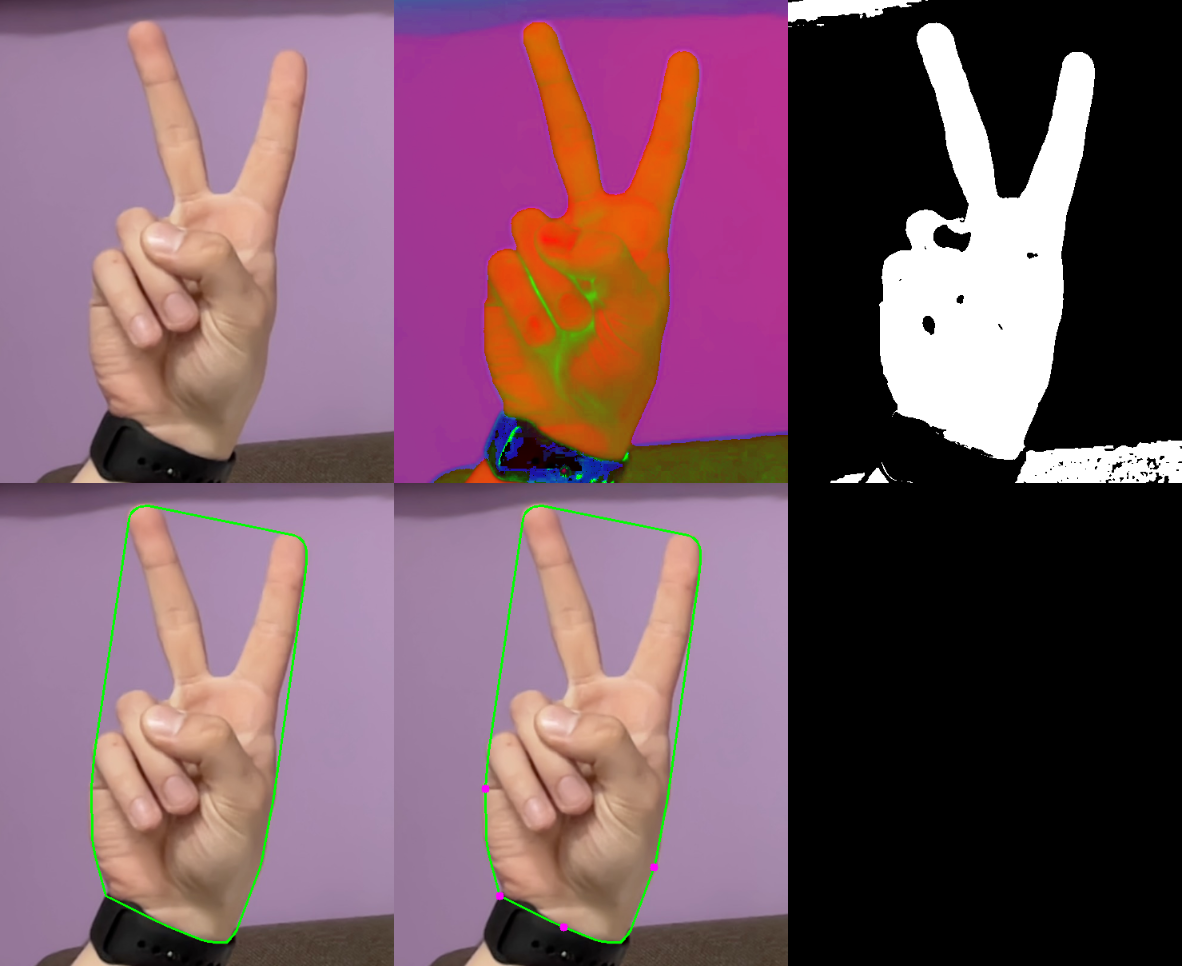
\includegraphics[width=\textwidth]{images/res_2_convex_hull_filter_1_y_2_x.png}
    \captionof{figure}{Résultat obtenus avec Convex Hull et filtrage des points}
    \label{fig:res_2_convex_hull_filter_1_y_2_x}
\end{center}

Là, nous nous sommes rendus compte qu'il y avait un problème avec le filtrage en y. Au lieu de garder les points 1.5 fois plus petits que la moyenne, nous avons décidé de garder les points 0.5 fois plus petits que la moyenne. \bigbreak

\begin{center}
    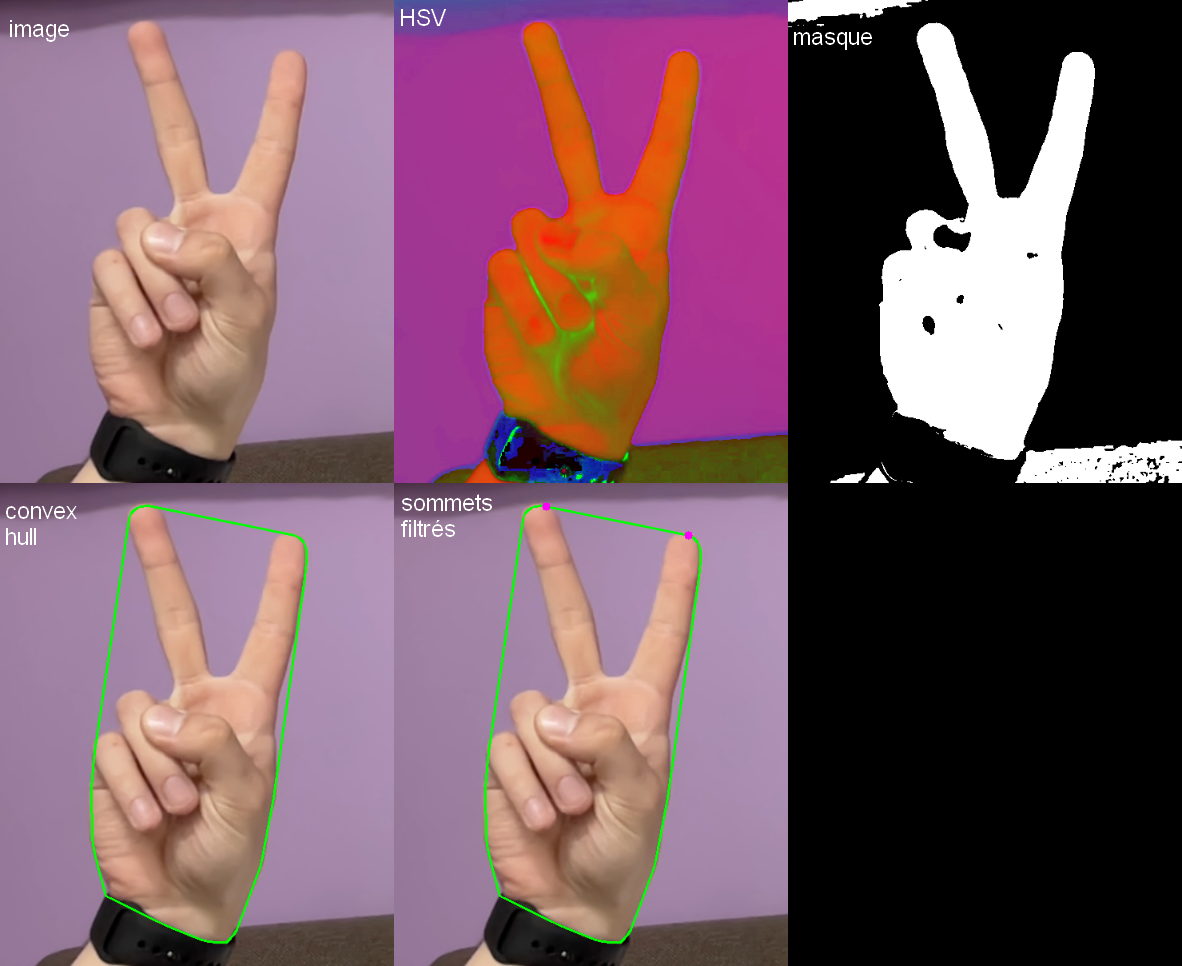
\includegraphics[width=\textwidth]{images/res_2_convex_hull_filter_2_y_2_x.png}
    \captionof{figure}{Résultat obtenus avec Convex Hull et filtrage des points}
    \label{fig:res_2_convex_hull_filter_2_y_2_x}
\end{center}

Là les résultats sont bons (Fig. \ref{fig:res_2_convex_hull_filter_2_y_2_x}). Nous avons bien deux points au bout de chaque doigts. \bigbreak

\begin{center}
    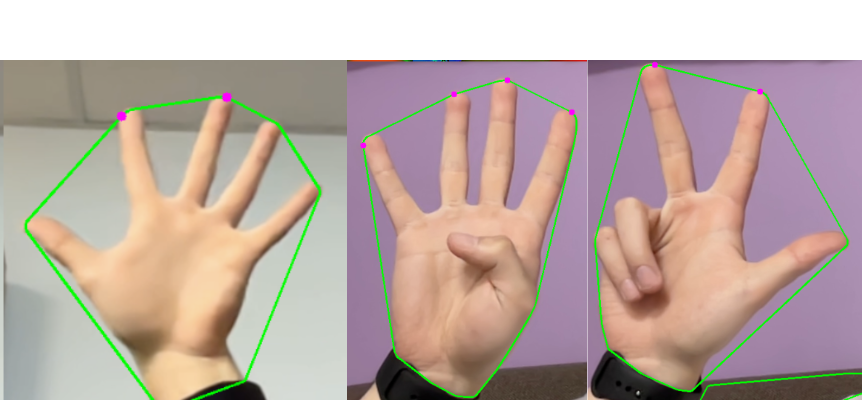
\includegraphics[width=\textwidth]{images/res_5_4_3_convex_hull_2_y_2x.png}
    \captionof{figure}{Résultat obtenus avec Convex Hull et filtrage des points}
    \label{fig:res_5_4_3_convex_hull_2_y_2x}
\end{center}

Nous avons donc re-tester avec ces nouveaux filtres sur plusieurs images avec 5, 4 et 3 doigts (Fig. \ref{fig:res_5_4_3_convex_hull_2_y_2x}). Les résultats ne sont pas aussi bons. En effet, nous pouvons voir qu'il n'y a que deux points sur l'image de 5 doigts et deux sur l'image de 3 doigts. 

\subsubsection{Conclusion}
Les résultats obtenus sont plutôt encourageants, nous avons réussi dans certains cas à détecter le bon nombre de doigts. Cependant, les résultats ne sont pas parfaits. En effet, les filtres que nous avons mis en place ne fonctionnent pas pour tous les cas : ils sont trop codés en durs pour s'appliquer à différents mouvements de la main. Il faudrait donc trouver une méthode pour que le programme puisse optimiser ces paramètres de manière autonome.

\section*{Conclusion}
\addcontentsline{toc}{section}{Conclusion}
En synthèse, notre exploration des méthodes de détection des mains et des doigts a révélé des résultats encourageants, bien que perfectibles. Malgré la configuration minutieuse des paramètres, la détection de la main a toutefois donné des résultats satisfaisants. Cependant, la reconnaissance des doigts se révèle être une tâche plus complexe. Il est essentiel de trouver une méthode permettant au programme d'optimiser ces paramètres de manière autonome, car les nombreux filtres nécessaires pour cette tâche sont très dépendants des caractéristiques des images. \bigbreak

Les réseaux de neurones apparaissent actuellement comme la méthode la plus prometteuse pour détecter les mouvements.Leur capacité à s'adapter à divers types d'images et à apprendre les meilleures représentations pour la détection des doigts offre un potentiel significatif pour améliorer la précision et la robustesse des systèmes de détection. \bigbreak

\newpage

\section*{Annexes}
\addcontentsline{toc}{section}{Annexes}

\section*{Bibliographie}
\addcontentsline{toc}{section}{Bibliographie}
\printbibliography

\newpage

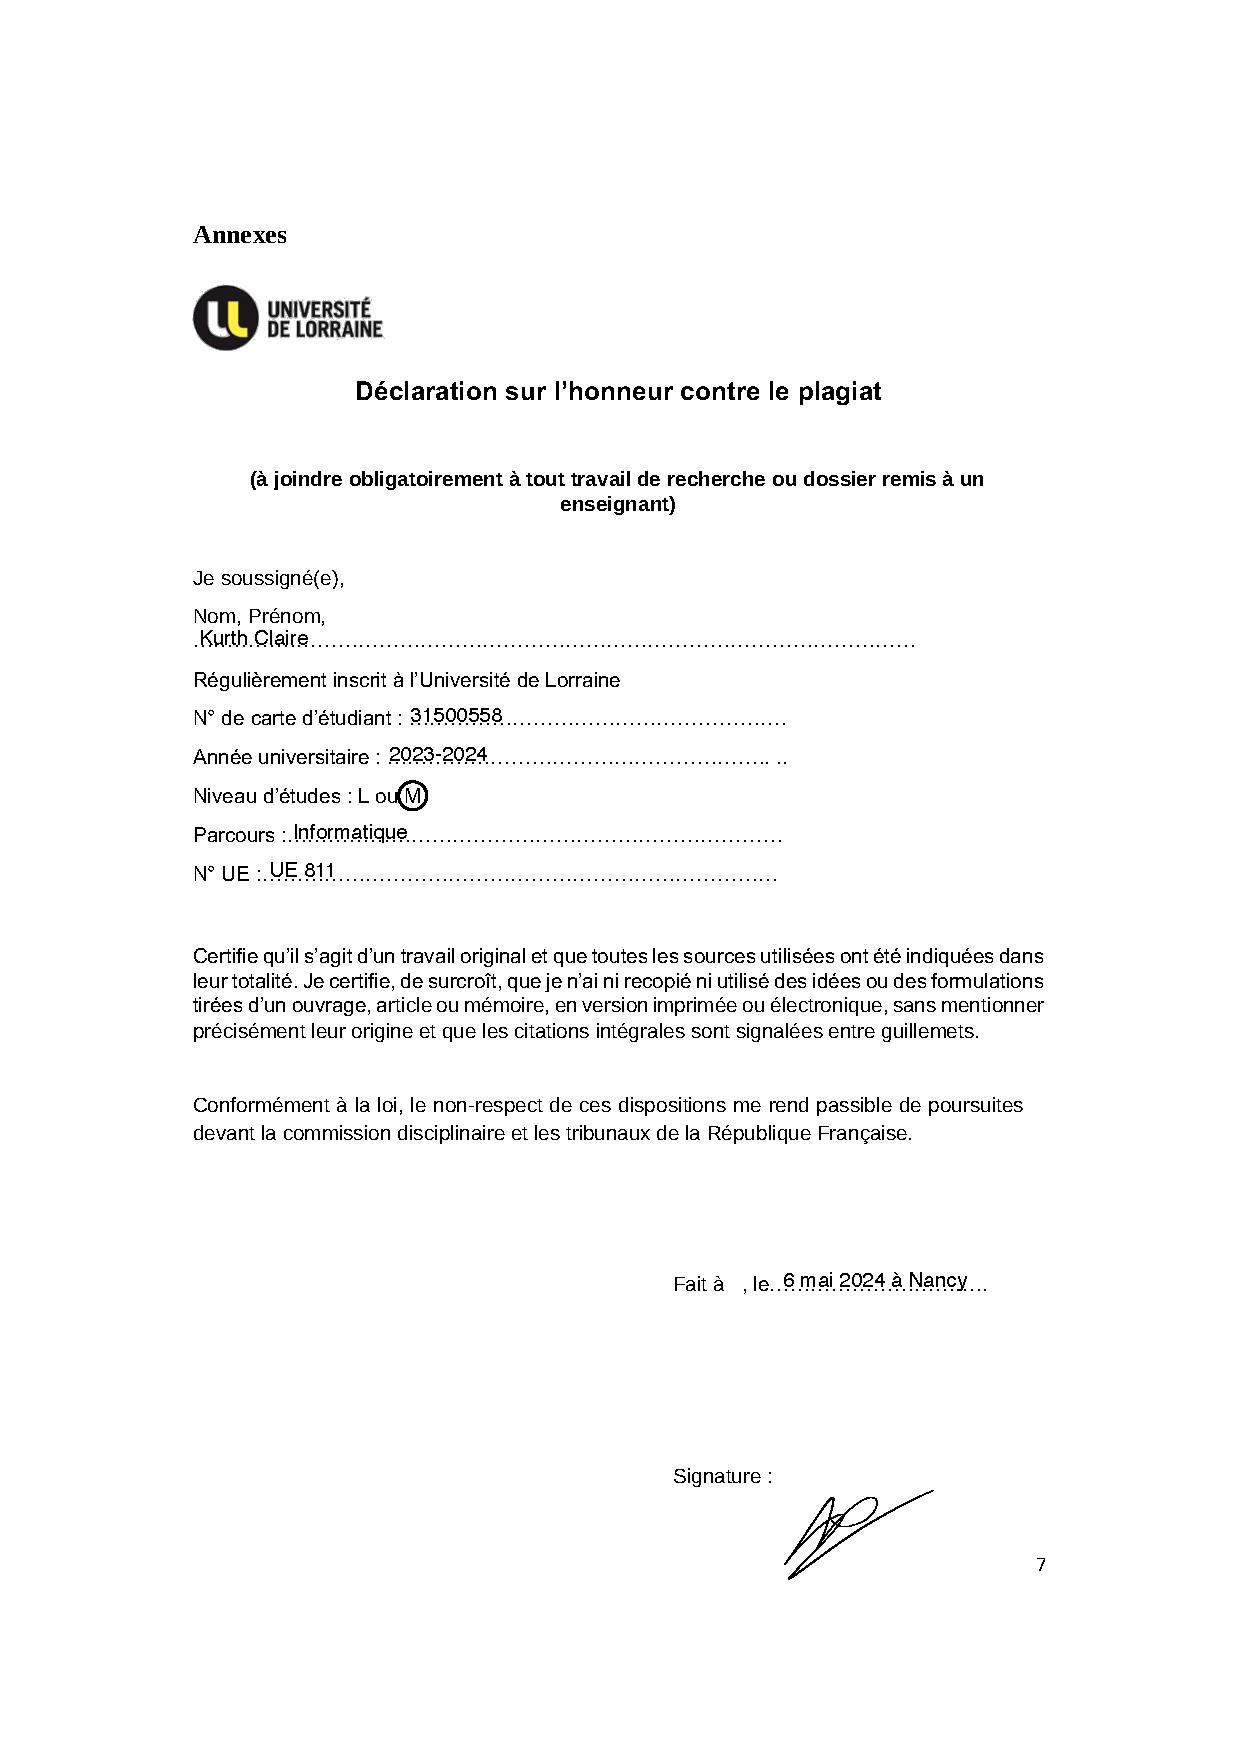
\includepdf{plagiat/declaration_plagiat_claire_out.pdf}
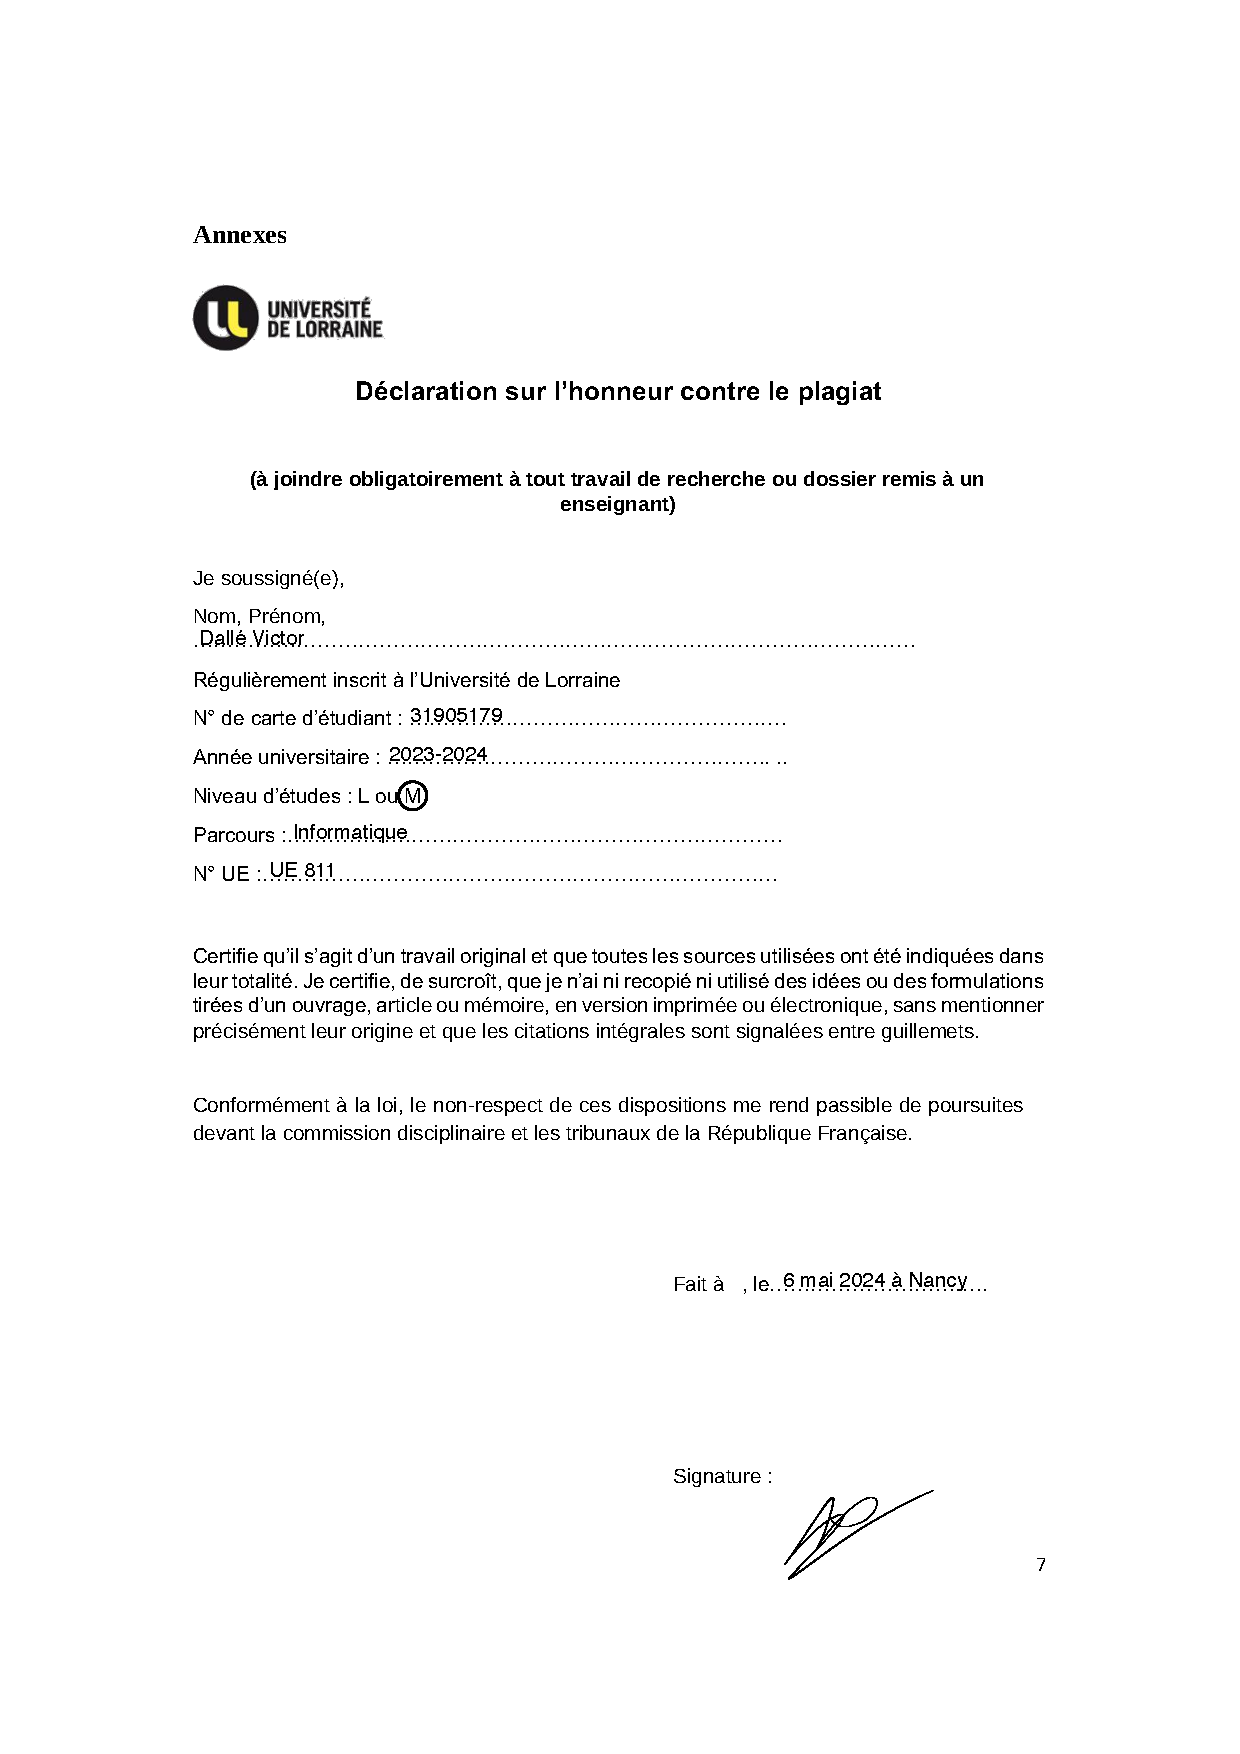
\includepdf{plagiat/declaration_plagiat_victor_out.pdf}

\newpage

\newpage
\section*{Résumé}

\end{document}